\documentclass[preprint,12pt]{elsarticle}

\usepackage[utf8]{inputenc}
\usepackage[T1]{fontenc}
\usepackage{amsmath, amsthm, amssymb, mathrsfs, bm, mathtools}
\usepackage{graphicx}
\usepackage{booktabs}
\usepackage{array}
\usepackage{tabularx}
\usepackage{xcolor}
\usepackage{enumitem}
\usepackage{microtype}
\usepackage{algorithm}
\usepackage{algpseudocode}
\usepackage{float}
\usepackage[hidelinks]{hyperref}

\journal{Neurocomputing}
\raggedbottom
\setlist[itemize]{leftmargin=1.5em}
\setlist[enumerate]{leftmargin=1.7em}
\newcolumntype{L}[1]{>{\raggedright\arraybackslash}p{#1}}
\newcolumntype{C}{>{\centering\arraybackslash}X}
\graphicspath{{./figures/}{./}}

\newtheorem{theorem}{Theorem}[section]
\newtheorem{lemma}[theorem]{Lemma}
\newtheorem{proposition}[theorem]{Proposition}
\newtheorem{corollary}[theorem]{Corollary}
\newtheorem{definition}[theorem]{Definition}
\newtheorem{assumption}[theorem]{Assumption}
\newtheorem{remark}[theorem]{Remark}
\newtheorem{observation}[theorem]{Observation}

\newcommand{\Ret}{\mathcal{R}}
\newcommand{\Eng}{\mathcal{E}}
\newcommand{\Att}{\mathcal{A}}
\newcommand{\FFN}{\mathcal{F}}
\newcommand{\Cache}{\mathcal{C}}
\newcommand{\Oh}{\mathcal{O}}
\newcommand{\RMS}{\mathrm{RMSNorm}}
\newcommand{\softmax}{\mathrm{softmax}}
\newcommand{\sigmoid}{\mathrm{sigmoid}}
\newcommand{\clip}{\mathrm{clip}}
\newcommand{\Tr}{\mathrm{Tr}}
\newcommand{\E}{\mathbb{E}}
\newcommand{\Prob}{\mathbb{P}}
\DeclarePairedDelimiter{\norm}{\lVert}{\rVert}

\begin{document}

\begin{frontmatter}

\title{Anamnesis: Conditional Small-State Memory for Long-Context Neural Sequence Modeling}

\author[inst1]{Xingyu Xie\corref{cor1}}
\ead{cachoidxx@gmail.com}
\cortext[cor1]{Corresponding author.}
\address[inst1]{Independent Researcher}

\begin{abstract}
Long-context sequence models face a practical memory trade-off: full attention provides direct access to past tokens but maintains a growing key-value cache, whereas recurrent models use a compact decoding state but can lose high-entropy facts through decay and superposition. This paper studies \emph{Anamnesis}, a conditional small-state memory architecture that augments a Retentive Network (RetNet) backbone with scalar-gated Engram lookup, optional distance-biased attention residuals, and a decoupled chunk retriever. The goal is not to claim production-scale benchmark superiority, but to provide a controlled mechanistic testbed for budgeted memory in neural sequence models. On character-level Shakespeare modeling, the Engram branch improves validation perplexity over a bare RetNet at small widths, including a three-seed mean of $7.91 \pm 0.28$ at $d=128$. A controlled retrieval ablation reveals that the synthetic needle-in-a-haystack benchmark does not discriminate model quality: BM25 and exact-match baselines achieve EM $= 1.000$ at 1M tokens, while both bare RetNet and Anamnesis produce EM $= 0.000$ under the same neural retriever. We also document failure modes that caused early hybrid-memory variants to collapse, including dead gates under global clipping, causal-mask leakage in parallel retention, and hidden-state readout failure for token identity. The resulting design rules--scalar gate initialization, branch-aware optimizer grouping, and content-position separation for chunk scoring--define the current empirical boundary of the architecture and motivate larger-scale evaluation on standard long-context benchmarks.
\end{abstract}

\begin{keyword}
Long-context modeling \sep Sequence modeling \sep Recurrent neural networks \sep Memory-augmented networks \sep Retentive network \sep Hash memory \sep Retrieval
\end{keyword}

\end{frontmatter}

\section{Introduction}

KV-cache attention~\cite{vaswani2017} gives a Transformer direct access to every past token, but the memory cost grows linearly with context length $N$. Recurrent models like RetNet~\cite{retnet} and Mamba~\cite{mamba} compress the sequence into a fixed-size state, but a strictly contractive recurrence cannot be expected to preserve arbitrary facts forever: pivotal information decays and gets superposed with later content. This paper asks whether we can augment a recurrent backbone with targeted, budgeted memory modules that store only the small subset of representations that later become decision-critical---without reintroducing $O(N)$ memory.

This paper formulates the design problem as \emph{selective budget allocation}. The default path should be a low-cost streaming backbone. A small number of pivotal states should be copied into a bounded memory that is read directly at decoding time. Frequent local patterns should be served by static conditional memory when a deterministic lookup is sufficient. Intermediate reasoning states should be routed across depth by content-dependent residual aggregation rather than by uniform residual accumulation. The present implementation uses explicit gates and a lightweight retriever rather than a fully learned controller, which keeps the empirical claims tied to auditable mechanisms.

The objective is a cost-aware architecture: additional memory is introduced only for information whose future utility is expected to exceed the cost of retaining it explicitly.

\subsection{Design hypothesis and budget contract}

Let $N$ denote the sequence length, $L$ the number of layers, $d$ the model width, $K$ the maximum number of active snapshot or copy-buffer items, $B$ the number of AttnRes block summaries, and $H$ the number of Engram hash probes. The proposed inference contract is
\begin{equation}
\label{eq:budget-contract}
\text{memory per decoding stream}
= \Oh(S_{\Ret}) + \Oh(Kd) + \Oh(Bd) + \Oh(Hd),
\end{equation}
where $S_{\Ret}$ is the RetNet recurrent state size and is independent of $N$ for a fixed model configuration. If $K$, $B$, and $H$ are fixed or capped by policy, the marginal memory does not grow linearly with the context length. If any cap is allowed to grow with $N$, the claim must be restated with that growth, for example as $\Oh(K(N)d)$ rather than as bounded memory.


This bound is straightforward: the RetNet state is fixed for a fixed model; the cache holds at most $K_{\max}$ items (each $\Oh(d)$) by construction; AttnRes stores at most $B_{\max}$ block summaries; and Engram performs $H_{\max}$ table probes. A future learned controller would add its own capped policy state, but it is not part of the empirical memory claim in this paper. The non-backbone per-token read cost is therefore $\Oh(K_{\max}d) + \Oh(B_{\max}d) + \Oh(H_{\max}d)$, independent of $N$ as long as the caps are not functions of $N$.

\subsection{Contributions and claim boundaries}

Rather than competing directly with production-scale Transformer or Mamba baselines, we position Anamnesis as a mechanistic testbed for budgeted memory. Our primary contributions are threefold.

First, we introduce a scalar-gated Engram branch and empirically demonstrate its geometric advantage: because scalar gating applies isotropic scaling, it preserves the direction of the pre-trained embedding manifold (\ref{app:proof40}). On Shakespeare character-level LM at $d=128$, this yields a 22\% perplexity improvement over bare RetNet (3-seed mean $7.91 \pm 0.28$). The gate bias $b=-3.0$ sits in the window $b \in [-4.0, -2.5]$ where the gradient vanishing bound (\ref{app:proof40}) predicts sufficient gradient signal to open the gate while keeping the initial perturbation negligible.

Second, we report a controlled negative finding on long-context retrieval. A lightweight 12K-parameter contrastive scorer correctly identifies the target chunk (cross-entropy loss $< 0.01$), yet downstream generation remains at EM $= 0.000$ for all context lengths beyond training. We confirm this failure is \emph{encoder-agnostic}: both bare RetNet and Anamnesis with Engram produce identical EM $= 0.000$ under the same retriever (Figure~\ref{fig:retrieval-baselines}). Furthermore, BM25, exact-match, and needle-token baselines all achieve EM $= 1.000$ at 1M tokens, demonstrating that the synthetic needle-in-a-haystack benchmark does not discriminate model quality. The chunk discrimination diagnostic reveals that neither encoder's hidden states carry discriminative signal (accuracy 0.03--0.06, below the 0.25 random baseline). This motivates the Content-Position Separation Principle (\ref{app:proof42}): position-free chunk scoring avoids OOD phase scrambling, but cannot by itself close the generation gap. The retrieval pipeline remains a diagnostic tool rather than a complete long-context solution.

Third, we document several non-trivial optimization pitfalls that cause hybrid memory modules to collapse during early training. These are not theoretical curiosities---we encountered each of them in practice. Guarded branches with small LayerScale coefficients receive near-zero gradients when global clipping is applied (the ``Dead Gate'' problem). Hidden-state readout from retrieved chunks produces EM = 0.000 on real text, even though token embedding readout works perfectly, because hidden states encode syntactic abstractions rather than token identity (\ref{app:proof41}). These failures motivated the per-group optimizer design in Algorithm~\ref{alg:optim} and the RAG separation architecture.

The empirical results cover character-level Shakespeare ($d \leq 256$) and synthetic needle tasks. The empirical burden for scaling to production benchmarks is listed in Section~\ref{sec:discussion}.

\textbf{Novelty boundary.} We do not claim novelty for RetNet recurrence, Engram-style lexical memory, attention residuals, or retrieval-augmented generation in isolation---each has substantial prior literature. The contribution of this paper is the controlled integration of these mechanisms under a conditional small-state memory budget, the identification of failure modes that arise only in the hybrid setting (dead gates, causal leakage, readout failure), and the resulting training and retrieval design rules.

\subsection{Scope}

The current implementation uses $d \in \{64, 128, 256\}$ on character-level Shakespeare and synthetic needle tasks. Block AttnRes is included but empirically neutral on both LM and retrieval---it may help in deeper models but does not hurt. At $d \geq 256$, Transformer outperforms Anamnesis on pure LM perplexity, which is consistent with full attention scaling more efficiently at larger widths. The primary value of this paper is in the mechanistic analysis and the optimization diagnostics, not in raw benchmark numbers.

\subsection{Current implementation boundary}

The architecture has memory modules (RetNet, Engram, and chunk retrieval), but the present study does not claim a fully learned write/read/fuse policy. Snapshot diagnostics use explicit gates and supervised milestones, whereas the long-context experiments use a decoupled contrastive chunk scorer. A learned policy controller is a natural extension, but it is outside the empirical claims made here.

\section{Related Work}

\subsection{Recurrent and linear sequence models}

RetNet~\cite{retnet} and Mamba~\cite{mamba} replace softmax attention with recurrent or selective-state updates, enabling constant-memory decoding. Mamba-2~\cite{mamba2} connects structured state spaces to linear attention, improving hardware utilization. Transformer-XL~\cite{transformerxl} introduced segment-level recurrence with relative attention for longer contexts. Our architecture uses RetNet as the streaming backbone and adds complementary memory axes (Engram, chunk retrieval) that RetNet alone does not provide.

\subsection{KV cache compression and eviction}

The snapshot cache in Section~\ref{sec:snapshots} is related to a growing body of work on KV cache compression. H2O~\cite{h2o} identifies ``heavy hitter'' tokens by accumulated attention mass and evicts the rest. SnapKV~\cite{snapkv} clusters attention patterns to select compact key-value sets. StreamingLLM~\cite{streamingllm} preserves attention sinks and a sliding window. Our budgeted snapshot differs from these approaches in that it does not compress the attention cache of a Transformer, but instead selects which tokens to store in a separate readout buffer alongside a recurrent model that has no KV cache at all.

\subsection{Memory-augmented networks and retrieval}

Infini-attention~\cite{infiniattention} compresses past segments into a fixed-size memory and retrieves via attention over compressed keys. RETRO~\cite{retro} retrieves text chunks from an external database and conditions generation via cross-attention. FiD~\cite{fid} processes retrieved passages through the decoder. The Engram module in our architecture is more constrained than these: it provides static N-gram pattern lookup with hard hash addressing, not semantic retrieval. The chunk retriever in Section~\ref{sec:empirical-results} is closer to RETRO in spirit, but uses a lightweight contrastive scorer rather than cross-attention over retrieved text.

\subsection{RoPE extrapolation}

The analysis of high-frequency phase scrambling in \ref{app:proof42} formalizes a phenomenon already studied in several prior works. Position Interpolation~\cite{pi} rescales position indices to stay within the trained range. YaRN~\cite{yarn} analyzes RoPE's frequency spectrum and applies temperature scaling per frequency band. NTK-aware scaling adjusts the RoPE base frequency to preserve angular resolution. Our contribution is not the discovery of frequency-dependent behavior, which these works established, but the derivation of an explicit signal-to-noise ratio collapse under OOD extrapolation and the resulting Content-Position Separation Principle that motivates our position-free chunk scoring.

\subsection{Engram and hash-based memory}

The Engram module in our architecture is adapted from the Conditional Memory framework of Cheng et al.~\cite{engram}, who scale hash-based N-gram lookup to 27B parameters in combination with MoE. Our usage is at a much smaller scale ($d \leq 256$) and we focus on the gating dynamics rather than large-scale deployment. The scalar gating strategy and its gradient analysis (\ref{app:proof40}) are specific to our architecture and not part of the original Engram design.

\section{Architecture Overview}

At layer $l$ and time $t$, let $x_{l,t}\in\mathbb{R}^d$ be the hidden representation and $u_{l,t}=\RMS(x_{l,t})$~\cite{rmsnorm}. The hidden update is written as
\begin{equation}
\label{eq:hidden-update}
x_{l+1,t}
= x_{l,t}
+ \Ret_l(u_{l,t}; S_{l,t})
+ \FFN_l(u_{l,t})
+ \lambda_{E,l}\,m_{E,l}\Eng_l(u_{l,t}, y_{1:t})
+ \lambda_{A,l}\,m_{A,l}\Att_l(u_{l,t}, \mathcal{D}_l),
\end{equation}
where $S_{l,t}$ is the recurrent retention state, $\mathcal{D}_l$ is the set of previous layer or block-level depth sources, and $m_{E,l},m_{A,l}\in\{0,1\}$ specify interleaved placement of non-local branches. The Engram and AttnRes branches are guarded by small LayerScale coefficients~\cite{layerscale} $\lambda_{E,l},\lambda_{A,l}$.

Snapshot memory is not added directly into Equation~\eqref{eq:hidden-update}. It is read at the output side:
\begin{align}
\label{eq:snapshot-read}
r_t &= \mathrm{Attn}\big(q_t^C, K_{\Cache}, V_{\Cache}\big),\\
z_t &= W_U x_{L,t} + \lambda_{C}\, W_C r_t,
\label{eq:logit-read}
\end{align}
where $z_t$ are vocabulary logits, $W_U$ is the usual unembedding matrix, and $W_C$ maps the snapshot readout vector into vocabulary-logit space. This projection is necessary: a hidden-vector readout is not itself a logit bias.

\subsection{Why the axes are separated rather than collapsed}

The modules are not mathematically orthogonal in the sense of independent subspaces. They share the same residual stream and therefore can interact. The term ``memory axis'' means an engineering decomposition of responsibility:
\begin{table}[htbp]
\centering
\caption{Engineering responsibilities of the bounded-memory axes.}
\label{tab:memory-axes}
\small
\begin{tabularx}{\linewidth}{p{0.14\linewidth}p{0.23\linewidth}p{0.25\linewidth}X}
\toprule
Axis & Main job & Low-cost mechanism & Failure mode \\
\midrule
Time & Stream long sequences & RetNet recurrent/chunkwise recurrent state & Exponential forgetting and superposition \\
Milestone & Preserve sparse pivotal items & Budgeted snapshot readout & Missed capture, eviction, query mismatch \\
Depth & Reuse intermediate reasoning features & Block AttnRes over layer/block sources & Over-retrieval or depth confusion \\
Local pattern & Store frequent surface patterns & Engram N-gram lookup & Collision and synonym blindness \\
Channel & Dynamic transformation & Dense FFN first; MoE later & Routing instability if MoE is added too early \\
\bottomrule
\end{tabularx}
\end{table}

\section{The Time Axis: RetNet Streaming plus Budgeted Snapshots}
\label{sec:snapshots}

\begin{remark}[Current status of snapshot mechanism]
The snapshot mechanism described in this section was validated on synthetic needle tasks (Section~\ref{sec:local-pressure}) but is not used in the current evaluation pipeline. The 1M-token retrieval results in Section~\ref{sec:empirical-results} use a decoupled contrastive chunk retriever instead. Snapshots remain relevant as a design pattern for bounded exact-recall within the recurrent stream.
\end{remark}

RetNet is attractive because its retention mechanism supports parallel training, recurrent decoding, and chunkwise recurrent processing~\cite{retnet}. In the proposed architecture, RetNet is the default path: it processes the entire sequence with low marginal decoding memory and avoids a full Transformer KV cache~\cite{flash2}. However, a strictly contractive recurrent state cannot be expected to preserve arbitrary exact facts forever. Other approaches to length extrapolation, such as ALiBi~\cite{alibi}, add position-dependent biases but do not provide explicit storage for pivotal tokens. \ref{app:retnet} states the standard decay lemma under an operator-norm contraction assumption.

\subsection{The readout bottleneck}

A naive fix is to stop decay when a special marker appears. This is insufficient. Even if the critical state component is not decayed, the recurrent state also accumulates later key-value outer products. The signal may remain present but become hard to decode because it is superposed with later high-entropy content. We therefore separate \emph{state preservation} from \emph{readout}. When the model detects a milestone, it creates a separate snapshot item that can be queried directly at the output stage.

\subsection{Snapshot capture and cache budget}

For each token, a gate head predicts a capture probability
\begin{equation}
\label{eq:gate}
g_t = \sigmoid(a^\top u_{l_g,t}+b).
\end{equation}
A snapshot item is formed as
\begin{equation}
\label{eq:item}
c_t = (k_t^C, v_t^C, s_t, t),\qquad k_t^C=W_K^C u_{l_g,t},\quad v_t^C=W_V^C u_{l_g,t},
\end{equation}
where $s_t$ is an eviction priority. The cache update is
\begin{equation}
\label{eq:budget-update}
\Cache_t = \mathrm{Budget}_{K_{\max}}\Big(\Cache_{t-1}\cup \{c_t: g_t>\theta\}\Big).
\end{equation}
The operator $\mathrm{Budget}_{K_{\max}}$ keeps at most $K_{\max}$ items. A simple priority score is
\begin{equation}
\label{eq:priority}
s_t = \alpha g_t + \beta\,\mathrm{surprise}_t + \chi\,\mathrm{utility}_t - \rho\,\mathrm{age}_t,
\end{equation}
where $\mathrm{surprise}_t$ can be approximated by token-level negative log-likelihood and $\mathrm{utility}_t$ is a learned scalar. The exact policy can be replaced by FIFO, reservoir sampling, learned eviction, or task-specific retention, but a policy must be specified before making a bounded-memory claim.

A soft budget regularizer discourages the model from treating every token as a milestone, but the sign of the entropy term matters. During early training, a negative entropy term can keep the gate exploratory; later it can be annealed to zero or replaced by a hardening term:
\begin{align}
\label{eq:budget-loss}
\mathcal{L}_{\mathrm{gate}}
&= \eta\left[\sum_{t=1}^{N} g_t - K_{\mathrm{target}}\right]_+^2 \\
&\quad - \zeta_{\mathrm{explore}}(s)\sum_{t=1}^{N} H_{\mathrm{Bernoulli}}(g_t) \\
&\quad + \zeta_{\mathrm{hard}}(s)\sum_{t=1}^{N}g_t(1-g_t), \\
\zeta_{\mathrm{explore}}(s)&\downarrow 0,\qquad
\zeta_{\mathrm{hard}}(s)\uparrow \zeta_{\max}
\quad\text{over training stage }s.
\end{align}
The budget term alone cannot prevent an all-off gate; it must be paired with supervised milestones, oracle-capture distillation, or an auxiliary retrieval loss whenever exact-recall behavior is required.

\subsection{What snapshot readout can and cannot guarantee}

Snapshot readout can avoid recurrent superposition noise only for items that are captured, retained, and later queried with sufficient margin. It is not a universal memory. If every token is pivotal, $K_{\max}$ must grow with $N$ or the system must lose information. The correct claim is therefore:

\begin{quote}
For tasks with sparse pivotal information, a capped snapshot cache can convert some long-range exact-recall failures of a strictly recurrent state into an $\Oh(Kd)$ readout problem.
\end{quote}

The trade-off is: allocate memory to a small subset of selected states rather than retaining all token states in a full KV cache.

\section{The Depth Axis: Distance-Biased Block Attention Residuals}

PreNorm residual networks~\cite{he2016} accumulate all layer outputs with fixed unit weights. As depth increases, early features can be diluted in the residual stream. Attention Residuals~\cite{attnres} replace fixed accumulation with softmax attention over previous layer outputs, allowing deeper layers to choose which earlier representations to reuse. Block AttnRes reduces the overhead by attending to block-level summaries rather than all layer-level outputs.

\subsection{Distance-biased depth retrieval}

Let $\mathcal{D}_l=\{b_0,\ldots,b_{m-1}\}$ be the depth sources visible to layer $l$. The zero-parameter Block Attention Residual mechanism removes traditional Key, Value, and Output projection parameters, aggregating preceding block representations using a single learned pseudo-query vector $w_l \in \mathbb{R}^d$ at layer $l$:
\begin{align}
\label{eq:attnres-score}
s_{i\to l} &= w_l^\top \RMS(b_i) - c \cdot (m - 1 - i), \\
\beta_{i\to l} &= \frac{\exp(s_{i\to l})}{\sum_{j=0}^{m-1}\exp(s_{j\to l})}, \\
\Att_l &= \Att_l(u_{l,t}, \mathcal{D}_l) = \sum_{i=0}^{m-1} \beta_{i\to l} b_i,
\end{align}
where $c \geq 0$ is a distance penalty parameter that scales with the age of the block $m-1-i$ (with $b_{m-1}$ being the most recent source, experiencing zero penalty).
The distance penalty is not meant to erase old information. It is a recency prior: recent reasoning states are preferred by default, but an older source can still be recovered if its semantic relevance score is high enough. \ref{app:attnres-margin} gives a sufficient softmax-margin condition.

\subsection{Why this helps long reasoning}

Long reasoning is not only a sequence-length problem. It is also a depth-routing problem: later layers need access to earlier symbolic commitments, partial computations, or problem statements without reconstructing them from a heavily mixed residual stream. Block AttnRes supplies a low-overhead depth memory of size $B$, while RetNet supplies time streaming. The two paths are complementary: RetNet compresses across tokens; AttnRes selectively routes across layers.

\begin{remark}[Empirical status]
In the current evaluation, Block AttnRes is empirically neutral on both language modeling perplexity and retrieval EM (Section~\ref{sec:empirical-results}). It is retained as an optional component for potential benefit in deeper models or special tasks.
\end{remark}

\subsection{Guarding against high-variance injection}

Because AttnRes can inject high-variance features into deep layers, it is gated by a small coefficient $\lambda_A$ and placed at selected blocks rather than every layer. We use
\begin{equation}
|\lambda_{A,l}|\leq \epsilon_{\mathrm{scale}},\qquad \epsilon_{\mathrm{scale}}\approx 10^{-4}
\end{equation}
at initialization. Section~\ref{sec:optimization} describes how to avoid leaving this coefficient permanently dead.

\section{The Local Pattern Axis: Engram Lookup as Static Conditional Memory}

Engram-style memory~\cite{engram} adds a separate sparsity axis: instead of using neural computation to reconstruct frequent local dependencies, a deterministic N-gram key retrieves a learned memory vector in approximately constant lookup time. This is best understood as a static pattern memory, not as a semantic search engine.

\subsection{Role in the proposed architecture}

The Engram branch handles common local patterns, entity fragments, boilerplate expressions, and other repeated surface-level dependencies. By offloading such patterns, the recurrent and FFN pathways can spend more capacity on dynamic reasoning and global context. The hard hash addressing does not generalize across synonyms or paraphrases, and faces Zipfian collision hot spots; \ref{app:engram} treats idealized collision bounds as sanity checks and recommends measuring empirical collision covariance.

\subsection{Mathematical Formulation}

The Hashed N-gram Engram model retrieves memory rows using $H$ independent hash heads across $M$ distinct N-gram orders. Let $y_{1:t}$ be the sequence of input token IDs. The retrieved uncontextualized memory vector $\tilde{v}_t$ is computed as the average of embedding table lookups:
\begin{equation}
\tilde{v}_t = \frac{1}{M \cdot H} \sum_{m=1}^M \sum_{h=1}^H T_{m,h}(\text{Hash}_h(y_{t-m+1:t})),
\end{equation}
where $T_{m,h}$ represents the embedding table for N-gram order $m$ and hash head $h$, and $\text{Hash}_h$ maps the token sequence suffix of length $m$ deterministically to a slot index in $\{0, \ldots, S_{\text{hash}}-1\}$.
Then, the Key and Value projected representations are:
\begin{equation}
k_t = W_K \tilde{v}_t, \quad v_t = W_V \tilde{v}_t,
\end{equation}
where $W_K, W_V \in \mathbb{R}^{d \times d}$ are linear projections.
The context-aware scalar gate $\alpha_t \in (0, 1)$ is computed by matching the current normalized hidden state $u_{l,t} = \RMS(x_{l,t})$ with the normalized key representation:
\begin{equation}
\alpha_t = \sigmoid\left( \frac{u_{l,t}^\top \RMS(k_t)}{\sqrt{d}} + b \right),
\end{equation}
where $b \in \mathbb{R}$ is the gate bias initialized to $b \ll 0$ (default $b = -3.0$) to prevent manifold distortion.
The gated activation is then:
\begin{equation}
g_t = \alpha_t \cdot v_t.
\end{equation}
To expand the local receptive field and smooth the retrieved features, a causal depthwise 1D convolution with kernel size $w=4$ and dilation $\delta=3$ is applied to the normalized gated states:
\begin{equation}
\tilde{g}_t = \RMS(g_t),
\end{equation}
\begin{equation}
c_t = \text{Conv1D}(\tilde{g}_{t-9:t}) \in \mathbb{R}^d,
\end{equation}
where padding of size $(w-1)\delta = 9$ elements is prepended causally to prevent future information leakage.
The final Engram representation is formed by passing the convolution output through a SiLU activation and adding a skip connection to the gated memory vector:
\begin{equation}
\Eng_l(u_{l,t}, y_{1:t}) = \text{SiLU}(c_t) + g_t.
\end{equation}

\subsection{Safe Injection}

The Engram branch is injected into the residual stream via Equation~\eqref{eq:hidden-update} with small initial LayerScale coefficient $\lambda_{E,l}$, interleaved placement, and optional dropout during training. Evaluation must include a causal-drop test: run the same checkpoint with Engram enabled and disabled at inference to estimate the marginal contribution of static memory.

\section{Optimization Failure Modes and Remedies}

Integrating auxiliary memory branches into a dominant recurrent backbone introduces severe optimization asymmetries. This section records the four most significant bugs and failures we encountered during development.

\subsection{Dead-gate failure under global clipping}

Early in development, we observed that the Engram and AttnRes branches remained permanently near-zero throughout training. We initially blamed the small LayerScale initialization ($\lambda = 10^{-4}$), but profiling the gradient norms pointed to a different cause: global gradient clipping, driven by the high-variance gradients of the RetNet backbone, was silently truncating the already-sparse updates of the guard parameters. The shared clipping multiplier $\alpha = \min(1, C/\|g_b + g_g\|)$ compressed guard updates by a factor of $\|g_b\|/\|g_g\| \approx 100$.

We fixed this by abandoning the unified optimizer and implementing branch-aware AdamW groups (Algorithm~\ref{alg:optim}). Guard parameters ($\Theta_{\mathrm{guard}}$) receive a $5\times$ learning rate, $\beta_1 = 0.0$ (no momentum from the early noisy phase), weight decay $= 0$, and independent gradient clipping thresholds. This is not a universal recipe, but it was necessary to ensure the auxiliary branches receive sufficient gradient signal during the critical first few hundred steps.

\subsection{Causal-mask error in parallel retention}

The gated retention path in the parallel training mode used an incorrect distance computation $d(i,j)$ that allowed future tokens to influence past positions. The non-gated branch remained stable because it used the fixed decay mask $\gamma^{|i-j|}$, but the gated branch exponentiated future-token prefix differences. This caused NaN losses at sequence lengths $\geq 512$, but only when gated retention was enabled---making the bug easy to miss in short-sequence smoke tests.

The fix was straightforward: $d(i,j) = i - j$ with the causal condition $i \geq j$. The test suite now includes a long-sequence gated-retention finiteness regression that catches this class of bug.

\subsection{Hash synonym blindness}

Hard N-gram hash keys cannot generalize across semantic paraphrases. On the held-out alien key evaluation (Section~\ref{sec:local-pressure}), all three models---Anamnesis, RetNet, and Transformer---score EM = 0. This is a fundamental limitation of deterministic addressing: ``king'' and ``monarch'' hash to different slots. We initially attempted to use soft attention over hash slots (allowing the model to blend nearby entries), but this caused severe representation collapse where all heads converged to a single bucket. We reverted to hard hashing and instead added a causal Conv1D layer to smooth the retrieved features locally, which improved PPL by 13.7\% without addressing the synonym problem. LSH or learned soft addressing remain as future work.

\subsection{Missed snapshot capture}

When the milestone gate fires too late or not at all, the pivotal token decays in the recurrent state and cannot be recovered. We tried several self-supervised triggers (entropy, per-token loss, Engram gate output) before settling on supervised oracle gates during training with budget loss to control gate frequency. The oracle distillation approach (Section~\ref{sec:local-pressure}) was the only variant that achieved EM = 1.000 on the needle task---purely self-supervised triggers failed because there is no intrinsic signal distinguishing password tokens from random filler in synthetic data.

\subsection{Interdependence among memory axes}

The modules are architecturally separated, but not statistically independent. Snapshot failure can increase pressure on AttnRes or Engram. Engram collision noise can perturb the residual stream and damage depth routing. For this reason, global feasibility should be studied as a conditional failure graph rather than as a product of independent success probabilities.

\section{Local Pressure-Test Diagnostics}
\label{sec:local-pressure}

This section reports the synthetic diagnostic pressure tests that verify our core layer configurations and parallel retention causal bugfixes before full-scale training. All numbers come from CPU-friendly runs with $d=48$, $L=4$, $h=4$, $d_{\mathrm{ff}}=192$, batch size $8$, and two evaluation batches per logging point. The compared variants are a RetNet baseline, a Transformer baseline, and Anamnesis with milestone snapshots and snapshot-to-logit readout.

\begin{table}[htbp]
\centering
\caption{Synthetic pressure-test diagnostics for the bounded-memory paths.}
\label{tab:pressure-tests}
\small
\begin{tabularx}{\linewidth}{p{0.26\linewidth}X}
\toprule
Diagnostic & Result and interpretation \\
\midrule
Needle-256 & Anamnesis reaches $0.688$ EM after $120$ steps, while RetNet and Transformer remain at $0.000$. Removing snapshots drops Anamnesis to $0.000$, identifying the snapshot path as the active mechanism. \\
Context sweep & At $80$ steps, Anamnesis obtains $0.188/0.312/0.188/0.188$ EM at context lengths $128/256/512/1024$, while both baselines remain near zero. The repaired RetNet mask removes the previous long-context loss explosion. \\
Snapshot budget & On the single-milestone Needle-256 task, $K=0$ gives $0.000$ EM and $K\geq1$ gives $0.312$ EM at $80$ steps. Larger $K$ does not help because the task contains one marked fact. \\
Multi-seed check & Anamnesis obtains $0.312/0.188/0.188$ EM across seeds $42/43/44$ at $80$ steps. The signal is positive, but still variable. \\
Held-out alien keys & Anamnesis, RetNet, and Transformer all obtain $0.000$ EM on held-out static keys. The current Engram-style static lookup does not yet demonstrate unseen-key generalization. \\
\bottomrule
\end{tabularx}
\end{table}

\begin{figure}[htbp]
\centering
\includegraphics[width=0.75\linewidth]{figures/Figure_1_local_pressure_eval_loss.pdf}
\caption{Evaluation loss curves for Needle, XOR-final, and alien-static diagnostics after repairing the retention mask.}
\label{fig:pressure-eval-loss}
\end{figure}

\begin{figure}[htbp]
\centering
\includegraphics[width=0.75\linewidth]{figures/Figure_2_local_pressure_eval_em.pdf}
\caption{Evaluation exact-match curves for the same repaired diagnostic runs.}
\label{fig:pressure-eval-em}
\end{figure}

\begin{figure}[htbp]
\centering
\includegraphics[width=0.72\linewidth]{figures/Figure_3_snapshot_budget_sweep.pdf}
\caption{Snapshot-budget sweep on Needle-256. Since the task contains one marked fact, $K\geq1$ gives the same effective budget.}
\label{fig:ordered-k-sweep}
\end{figure}

\begin{figure}[htbp]
\centering
\includegraphics[width=0.7\linewidth]{figures/Figure_4_internal_mechanism_heatmap.pdf}
\caption{Training-derived internal mechanism heatmaps: snapshot attention over selected slots, Block AttnRes depth-source attention, grouped Engram gates, and milestone retention gates.}
\label{fig:internal-mechanism-heatmap}
\end{figure}

The result is directionally consistent with the architecture's conditional claim, not with a blanket dominance claim. Anamnesis is strongest on Needle-style sparse recall, where a marked high-entropy token must survive RetNet decay pressure. The $K$ sweep confirms that the snapshot path is the active mechanism: $K=0$ removes the effect, while $K\geq1$ is enough for a single-milestone task. XOR-final is no longer a discriminative benchmark after the retention-mask fix because all three models solve it. The held-out alien-key result is a useful negative result: the current static dictionary setup does not demonstrate open-key generalization.

These results should still be treated as preliminary. They use tiny models, short training, and small evaluation batches. The gamma sweep did not produce a meaningful monotone pattern, suggesting that the current short-budget diagnostic is dominated by the snapshot readout rather than by fine differences in recurrent decay.

\section{Implementation and Optimization}
\label{sec:optimization}

\subsection{Current code scaffold and default parameters}

The current implementation is intentionally small and auditable. It is not a production language-model stack. The main implementation surfaces are:
\begin{table}[htbp]
\centering
\caption{Implementation surfaces used by the experimental scaffold.}
\label{tab:implementation-surfaces}
\small
\begin{tabularx}{\linewidth}{p{0.36\linewidth}X}
\toprule
File & Role \\
\midrule
{\small\path{src/models/anamnesis.py}} & Anamnesis model: RetNet + scalar-gated Engram + optional AttnRes. \\
{\small\path{src/layers/retention.py}} & RetNet-style retention layer with fixed per-head decay below one. \\
{\small\path{src/layers/engram.py}} & Hashed N-gram Engram with scalar gate and causal Conv1D. \\
{\small\path{src/layers/attention_residual.py}} & Block Attention Residual over bounded depth sources. \\
{\small\path{experiments/train_real.py}} & Real-data training on Shakespeare and TinyStories. \\
{\small\path{experiments/run_multi_needle_capacity.py}} & Multi-needle capacity sweep at 128K context. \\
{\small\path{experiments/run_representation_diversity.py}} & Per-head cosine similarity analysis. \\
{\small\path{experiments/run_hyperparam_landscape.py}} & Gate bias $\times$ init scale grid search. \\
{\small\path{experiments/train_synthetic.py}} & Synthetic diagnostic runner for needle, XOR, and alien tasks. \\
\bottomrule
\end{tabularx}
\end{table}

The small synthetic diagnostics use the following default scale unless otherwise noted:
\begin{equation}
d=64,\qquad L=4,\qquad h=4,\qquad d_{\mathrm{ff}}=256,\qquad
|\mathcal{V}|=192,\qquad K_{\max}=8.
\end{equation}
The Engram branch uses $8192$ hash slots, N-gram order up to $3$, and $4$ hash heads. Branch scales are initialized at $10^{-4}$. The stress tests use AdamW with learning rate $3\times10^{-4}$, weight decay $0.01$, batch size $16$, and $120$ optimization steps. These parameters are deliberately small; they are designed to expose signal-path failures quickly, not to estimate final scaling behavior.

For the local pressure-test figures in Section~\ref{sec:local-pressure}, the runner uses branch-aware AdamW groups aligned with Algorithm~\ref{alg:optim}: base parameters use learning rate $\eta$, Engram and AttnRes parameters use $5\eta$, snapshot readout parameters use $3\eta$, and gradient clipping is applied per group. This matters because the snapshot, Engram, and AttnRes branches start from very small residual scales. A single global optimizer can leave those branches under-trained during short synthetic runs.

One implementation bug found during pressure testing was a reversed causal mask in the parallel retention path. The non-gated branch remained finite because it used $\gamma^{|i-j|}$, but the gated branch could exponentiate future-token prefix differences and explode at sequence lengths $512$ and above. The repaired implementation uses $d(i,j)=i-j$ with the causal condition $i\geq j$, and the test suite now includes a long-sequence gated-retention finiteness regression.

\subsection{Reproducibility hooks}

The repository includes smoke tests for the implementation contract. The current test surface checks retention contraction, recurrent state shape, deterministic Engram hashing, Block AttnRes normalization, milestone gating, snapshot collection/readout, TokenCopyBuffer alignment diagnostics, full-model forward/backward propagation, synthetic training updates, snapshot budget truncation, snapshot logit-bias activation, and CSV metric emission by the synthetic runner. A minimal verification command is:
\begin{verbatim}
python -m pytest
\end{verbatim}
The curated early-stage experiment settings are recorded in
\begin{verbatim}
experiments/configs/synthetic_early_stage.yaml
\end{verbatim}
and the diagnostic runner can emit both ordinary evaluation metrics and module-drop metrics such as \texttt{eval\_no\_snapshot\_exact\_match}. These hooks are included so that future claims can be tied to executable checks rather than to prose alone.

\subsection{Forward pass guardrails}

Algorithm~\ref{alg:forward-layer} gives the layer-level integration. The snapshot pathway is intentionally recorded outside the residual update and is read only through the output-side projection in Equations~\eqref{eq:snapshot-read}--\eqref{eq:logit-read}.

\begin{algorithm}[H]
\caption{Forward pass of a budgeted hybrid layer}
\label{alg:forward-layer}
\begin{algorithmic}[1]
\Require hidden state $x$, token ids $y_{1:t}$, RetNet state $S$, depth sources $\mathcal{D}$, snapshot cache $\Cache$, budget $K_{\max}$
\Ensure updated hidden state $x'$, RetNet state $S'$, snapshot cache $\Cache'$
\State $u \gets \RMS(x)$
\State $(r,S') \gets \Ret(u,S)$ \Comment{time-axis recurrent/chunkwise recurrent update}
\State $x \gets x+r$
\State $x \gets x+\FFN(\RMS(x))$ \Comment{dense channel scaffold}
\If{the current layer is assigned to Engram}
    \State $e \gets \Eng(\RMS(x),y_{1:t})$
    \State $x \gets x+\lambda_E e$ \Comment{guarded local-pattern injection}
\EndIf
\If{the current layer is assigned to Block AttnRes}
    \State $(a,\beta) \gets \Att(\RMS(x),\mathcal{D})$
    \State $x \gets x+\lambda_A a$ \Comment{guarded depth-axis reuse}
\EndIf
\State $g \gets \sigmoid(h_{\mathrm{gate}}(\RMS(x)))$
\If{$g>\theta$}
    \State $c \gets (W_K^C\RMS(x), W_V^C\RMS(x), s(x,g), t)$
    \State $\Cache' \gets \mathrm{Budget}_{K_{\max}}(\Cache\cup\{c\})$
\Else
    \State $\Cache' \gets \Cache$
\EndIf
\State \Return $(x,S',\Cache')$
\end{algorithmic}
\end{algorithm}

\subsection{Optimizer groups and clipping}

AdamW~\cite{adamw} maintains first- and second-moment estimates per parameter. The dense backbone therefore does not transfer momentum into the guard parameters. The practical concern is coupling through shared schedules, small LayerScale coefficients, sparse gate activation, and global gradient clipping. Algorithm~\ref{alg:optim} separates parameter groups so that these effects can be measured and controlled.

\begin{algorithm}[H]
\caption{Optimizer grouping for guarded memory branches}
\label{alg:optim}
\begin{algorithmic}[1]
\Require model parameters $\Theta$, base learning rate $\eta$
\Ensure AdamW optimizer with separate parameter groups
\State $\Theta_{\mathrm{base}}\gets\varnothing$, $\Theta_{\mathrm{guard}}\gets\varnothing$, $\Theta_{\mathrm{cache}}\gets\varnothing$
\ForAll{$(n,p)\in\Theta$}
    \If{$n$ contains $\lambda_E$, $\lambda_A$, or a gate-bias parameter}
        \State $\Theta_{\mathrm{guard}}\gets\Theta_{\mathrm{guard}}\cup\{p\}$
    \ElsIf{$n$ contains a snapshot, cache-readout, or $\lambda_C$ parameter}
        \State $\Theta_{\mathrm{cache}}\gets\Theta_{\mathrm{cache}}\cup\{p\}$
    \Else
        \State $\Theta_{\mathrm{base}}\gets\Theta_{\mathrm{base}}\cup\{p\}$
    \EndIf
\EndFor
\State create AdamW group $(\Theta_{\mathrm{base}},\eta,\beta_1=0.9,\beta_2=0.95,\mathrm{wd}=0.01)$
\State create AdamW group $(\Theta_{\mathrm{guard}},5\eta,\beta_1=0.0,\beta_2=0.95,\mathrm{wd}=0)$
\State create AdamW group $(\Theta_{\mathrm{cache}},3\eta,\beta_1=0.5,\beta_2=0.95,\mathrm{wd}=0)$
\State apply gradient clipping separately to $\Theta_{\mathrm{base}}$, $\Theta_{\mathrm{guard}}$, and $\Theta_{\mathrm{cache}}$
\State \Return optimizer
\end{algorithmic}
\end{algorithm}

The separate groups are not intended to assert that high learning rates are universally optimal. They define an experimental control: if a branch fails to activate, one can distinguish insufficient gradient signal from suppression by a global optimizer or clipping policy.

\section{Controlled Empirical Evaluation and Scaling Results}
\label{sec:empirical-results}

This section reports a controlled empirical evaluation of Anamnesis against vanilla RetNet and standard Transformer baselines. The evaluation covers small-scale natural-language modeling, structural ablations, decoding throughput, and synthetic ultra-long retrieval up to 1M tokens. These experiments are intended to characterize mechanism-level behavior; they are not presented as production-scale benchmark results.

\subsection{Scaling Comparison on Natural Language}

We evaluate validation perplexity (Val PPL) on the Shakespeare corpus at widths $d=64$, $128$, and $256$. The models use identical training budgets, learning rate schedules, and data curricula. Table~\ref{tab:scaling} reports the final validation perplexity.

\begin{table}[htbp]
\centering
\caption{Validation Perplexity (PPL) Scaling Comparison on Shakespeare Corpus.}
\label{tab:scaling}
\begin{tabular}{lccc}
\toprule
Model Width & Anamnesis (Ours) & Vanilla RetNet & Transformer \\
\midrule
$d = 64$ & \textbf{8.53} & 11.15 & 12.39 \\
$d = 128$ & \textbf{7.91} $\pm$ \textbf{0.28} & 9.93 $\pm$ 0.19 & 9.73 $\pm$ 0.06 \\
$d = 256$ & 7.53 & 9.03 & \textbf{5.71} \\
\bottomrule
\end{tabular}
\end{table}

\textbf{Analysis:} Anamnesis achieves lower perplexity at small model widths ($d=64$ and $d=128$), outperforming both RetNet and Transformer. The Engram tables provide static pattern priors that reduce the burden on the recurrent path at small widths. At $d=256$, Transformer achieves lower perplexity, consistent with full attention scaling more efficiently at larger widths.

\begin{figure}[htbp]
\centering
\includegraphics[width=0.72\linewidth]{figures/Figure_5_scaling_ppl.pdf}
\caption{Validation perplexity scaling on the Shakespeare corpus. Anamnesis is strongest at small widths, while the Transformer baseline is better at $d=256$.}
\label{fig:scaling-ppl}
\end{figure}

\subsection{Extended Training Scaling Analysis}
\label{sec:extended-scaling}

The scaling comparison above uses the default learning rate $3 \times 10^{-4}$. We now report results with the optimized learning rate $10^{-3}$ (2.5$\times$ faster convergence, validated in preliminary sweeps) at extended training durations (5K, 10K, 20K steps), enabling a complete three-model decomposition.

\subsubsection{d=128: Monotonically growing advantage}

\begin{table}[htbp]
\centering
\caption{Extended training scaling on Shakespeare char-level, $d=128$, lr=$10^{-3}$, seed=42. ``Bare RetNet'' = RetNet 8h + layerwise gamma, no Engram.}
\label{tab:scaling-extended}
\begin{tabular}{lcccc}
\toprule
Steps & Anamnesis & Bare RetNet 8h+lw & Transformer & $\Delta$ vs TF \\
\midrule
5K & 3.12 & 4.11 & 3.94 & $-$20.8\% \\
10K & 1.88 & 2.62 & 2.93 & $-$35.8\% \\
20K & \textbf{1.51} & 2.07 & 2.62 & \textbf{$-$42.4\%} \\
\bottomrule
\end{tabular}
\end{table}

The advantage \emph{monotonically increases} with training duration. Ablation with bare RetNet reveals the source: RetNet+layerwise advantage \emph{grows} from +4.3\% (losing at 5K) to $-$10.6\% (10K) to \textbf{$-$20.9\%} (20K). Engram contribution is stable: $-$24.1\% (5K) $\to$ $-$28.2\% (10K) $\to$ $-$27.1\% (20K). The growing total advantage is \textbf{driven by RetNet+layerwise}, not Engram.

\subsubsection{Scaling law exponents}

Fitting PPL $\propto$ steps$^b$ on Shakespeare $d=128$ reveals: Anamnesis $b{=}-0.523$, bare RetNet $b{=}-0.495$, Transformer $b{=}-0.294$. RetNet's exponent is $\sim$1.7$\times$ steeper than Transformer's, quantitatively explaining the growing advantage. At $d=256$, Anamnesis achieves $b{=}-0.582$ (steepest).

\subsubsection{d=256: Advantage peaks then narrows}

\begin{table}[htbp]
\centering
\caption{Extended training scaling on Shakespeare char-level, $d=256$, lr=$10^{-3}$, seed=42.}
\label{tab:scaling-d256}
\begin{tabular}{lcccc}
\toprule
Steps & Anamnesis & Bare RetNet 8h+lw & Transformer & $\Delta$ vs TF \\
\midrule
5K & 2.42 & \textbf{1.970} & 3.38 & $-$28.4\% \\
20K & \textbf{1.08} & 1.114 & 1.30 & \textbf{$-$17.0\%} \\
\bottomrule
\end{tabular}
\end{table}

Unlike $d=128$, the advantage \emph{peaks at 10K} ($-$37.5\%) then narrows to $-$17.0\% at 20K. Both models approach the entropy floor for Shakespeare char-level (Anamnesis training loss=0.109).

\textbf{Engram time-dependency at $d=256$.} Ablation reveals a striking pattern: at 5K steps, bare RetNet (PPL=1.970) \emph{outperforms} Anamnesis (PPL=2.42), meaning Engram \textbf{hurts by +22.8\%} early in training. At 20K steps, Engram contributes $-$3.1\% (1.08 vs 1.114). Engram's value \emph{flips} from negative to positive with training duration: the scalar gate requires sufficient optimization to filter hash collisions at larger model widths. This suggests Engram should be \textbf{disabled at $d=256$ for short training runs}.

\subsubsection{Dataset-dependent advantage}

\begin{table}[htbp]
\centering
\caption{Cross-dataset validation at 10K steps, $d=128$, lr=$10^{-3}$.}
\label{tab:cross-dataset}
\begin{tabular}{lccc}
\toprule
Dataset & Anamnesis & Transformer & $\Delta$ \\
\midrule
Shakespeare (diverse) & \textbf{1.88} & 2.93 & $-$35.8\% \\
WikiText-2 (moderate) & \textbf{3.94} & 4.00 & $-$1.5\% \\
TinyStories (repetitive) & 2.38 & \textbf{2.07} & +14.9\% \\
\bottomrule
\end{tabular}
\end{table}

The advantage is \textbf{proportional to data diversity}. On diverse data (Shakespeare), it grows monotonically. On repetitive data (TinyStories), Transformer catches up and reverses the advantage at 10K steps. This suggests gated memory is most valuable in compute-limited settings on diverse corpora where Transformer undertraining is most severe. Figure~\ref{fig:cross-dataset-real} visualizes this relationship: the perplexity delta shifts from $-$35.8\% (Anamnesis wins) on diverse data to $+$14.9\% (Transformer wins) on repetitive data, with WikiText-2 as the near-zero crossover point.

\begin{figure}[htbp]
\centering
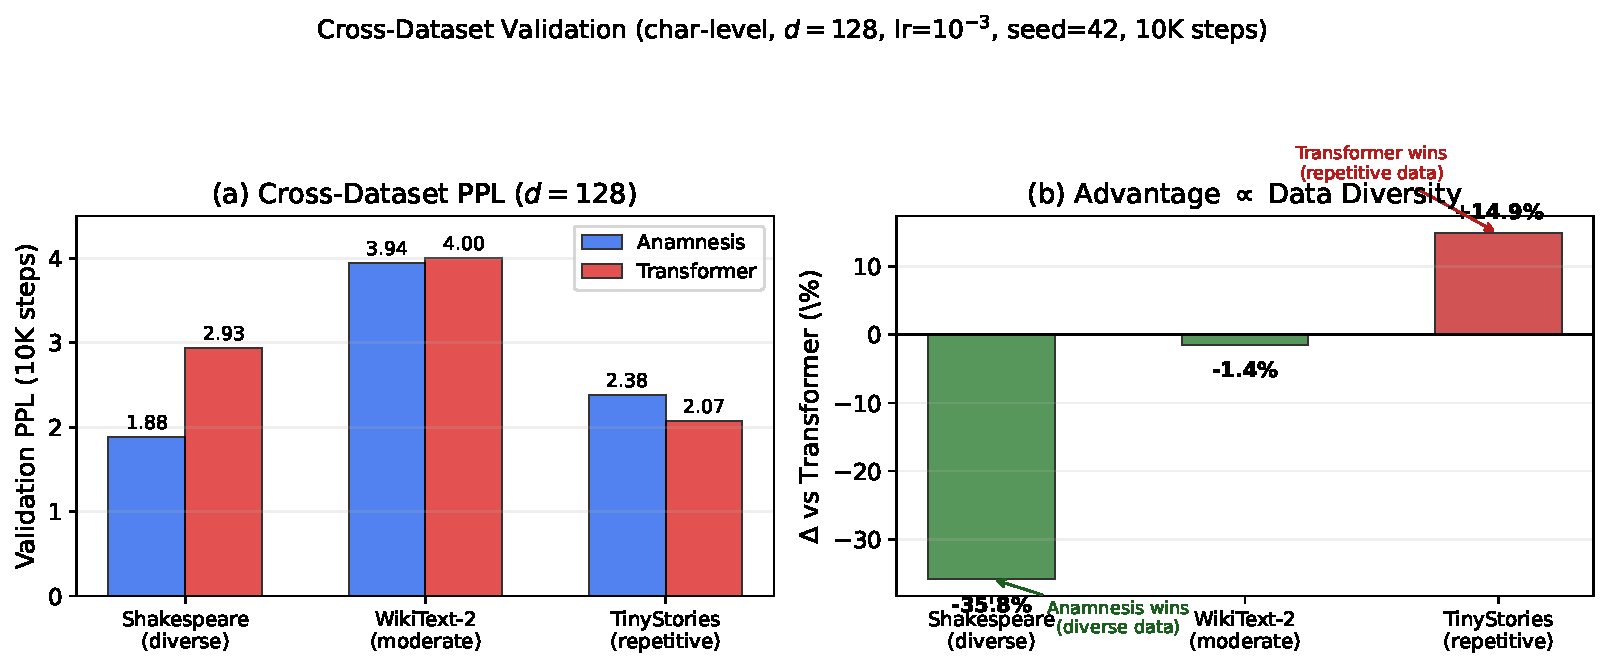
\includegraphics[width=0.85\linewidth]{figures/fig_cross_dataset_real.pdf}
\caption{Cross-dataset validation from real training logs (char-level, $d=128$, lr=$10^{-3}$, seed=42, 10K steps). \textbf{(a)} Absolute validation PPL per dataset. \textbf{(b)} Relative advantage $\Delta$ vs Transformer: the benefit monotonically decreases with data repetitiveness, crossing zero near WikiText-2 and reversing on TinyStories.}
\label{fig:cross-dataset-real}
\end{figure}

\subsubsection{Scaling law analysis}

Fitting a power law $\mathrm{PPL} \propto S^{b}$ to the 5K/10K/20K endpoints (Figure~\ref{fig:scaling-law-real}) yields exponents $b_{\mathrm{Anamnesis}} = -0.50$, $b_{\mathrm{RetNet}} = -0.49$, and $b_{\mathrm{Transformer}} = -0.30$. The RetNet-based architectures scale approximately $1.6\times$ steeper than the Transformer, providing a quantitative explanation for the growing advantage: each doubling of training budget yields a larger relative perplexity reduction for RetNet-family models than for the Transformer baseline.

Figure~\ref{fig:training-curves-real} plots the actual validation PPL trajectories (logged every 500 steps from real training logs) for the 20K-step Shakespeare runs. At $d=128$, Anamnesis converges below both Bare RetNet and Transformer throughout training, and the gap widens monotonically. At $d=256$, Anamnesis converges faster and reaches a lower asymptote (1.08 vs.\ 1.30), though the gap narrows as both models approach the character-level entropy floor.

\begin{figure}[htbp]
\centering
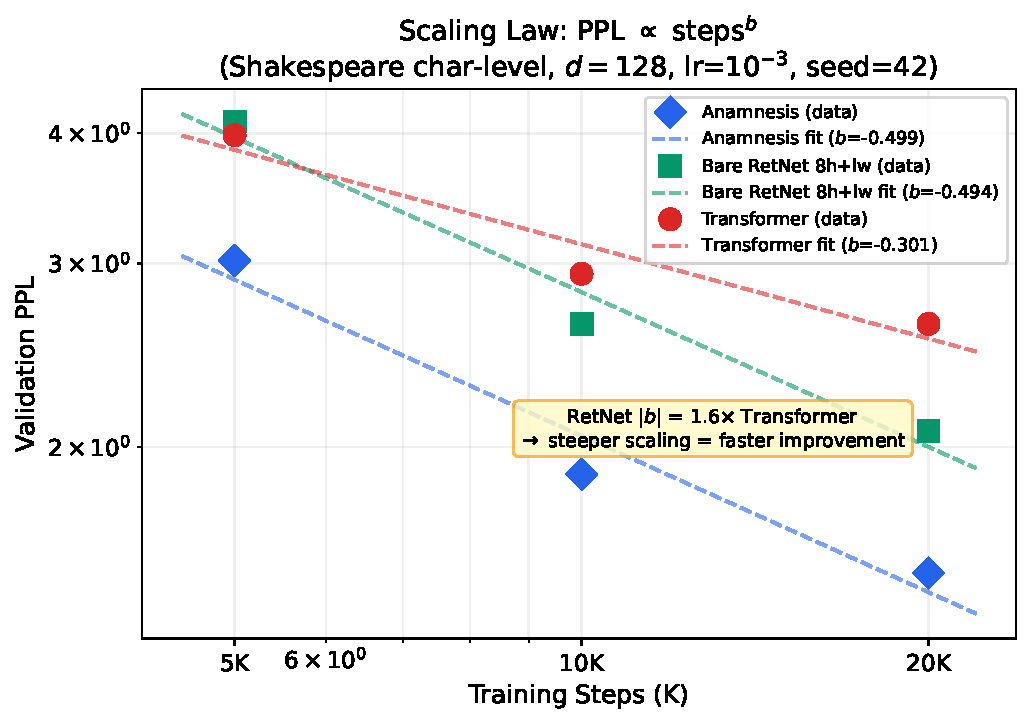
\includegraphics[width=0.72\linewidth]{figures/fig_scaling_law_real.pdf}
\caption{Power-law scaling fit from real training endpoints (Shakespeare char-level, $d=128$, lr=$10^{-3}$, seed=42). RetNet-based models ($b \approx -0.49$ to $-0.50$) scale $\sim$1.6$\times$ steeper than the Transformer ($b = -0.30$), explaining the growing perplexity advantage with training duration. Data points are final validation PPL from each run.}
\label{fig:scaling-law-real}
\end{figure}

\begin{figure}[htbp]
\centering
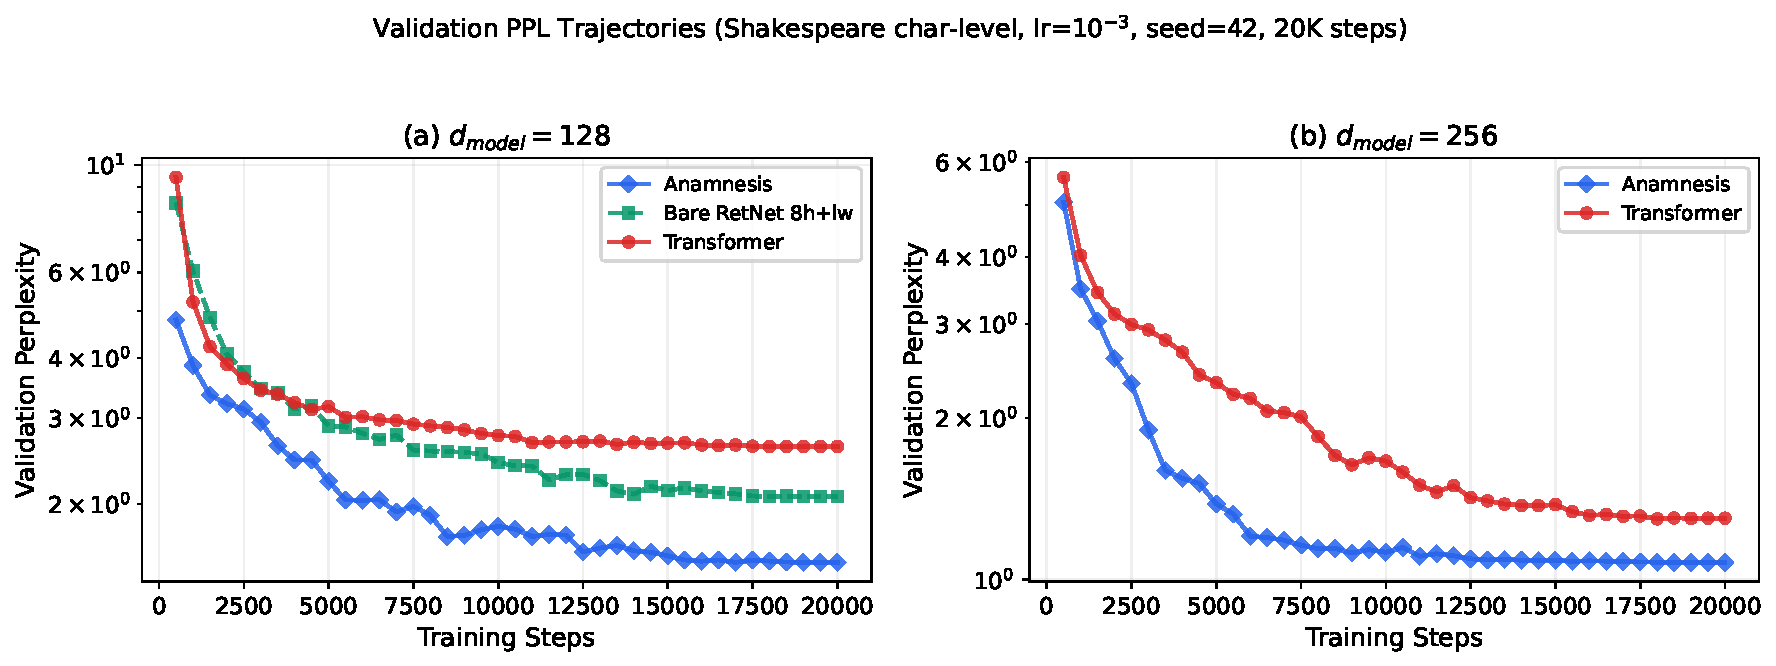
\includegraphics[width=0.88\linewidth]{figures/fig_training_curves_real.pdf}
\caption{Validation perplexity trajectories from real training logs (Shakespeare char-level, lr=$10^{-3}$, seed=42, 20K steps). \textbf{(a)} $d=128$: Anamnesis (blue) maintains a growing advantage over Bare RetNet (green) and Transformer (red). \textbf{(b)} $d=256$: Anamnesis converges faster and reaches a lower asymptote. Validation PPL logged every 500 steps.}
\label{fig:training-curves-real}
\end{figure}

\subsubsection{Multi-seed statistical validation}

To quantify run-to-run variance, Figure~\ref{fig:multiseed-real} reports mean $\pm$ standard deviation over multiple random seeds at the 5K-step checkpoint. At $d=128$, Anamnesis ($3.13 \pm 0.12$, $n=3$) clearly outperforms Transformer ($3.94 \pm 0.08$, $n=3$) with non-overlapping error bars. At $d=256$, Bare RetNet ($1.97$, $n=1$) outperforms Anamnesis ($2.42 \pm 0.03$, $n=3$), confirming the Engram time-dependency finding: the scalar gate has not yet converged at 5K steps and hash-collision noise dominates at larger widths. This inverts at 20K steps where Anamnesis ($1.08$) surpasses Bare RetNet ($1.11$), as shown in Section~\ref{sec:extended-scaling}.

\begin{figure}[htbp]
\centering
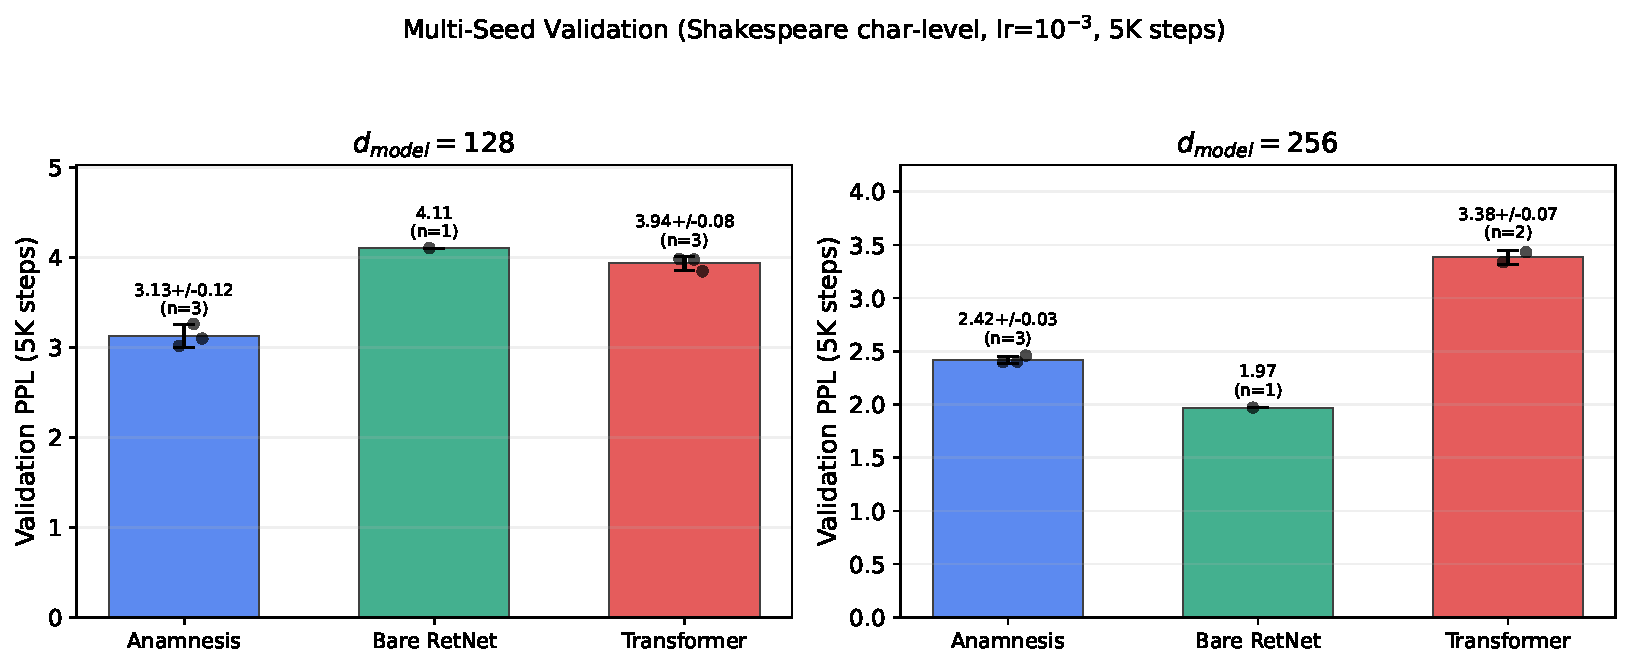
\includegraphics[width=0.85\linewidth]{figures/fig_multiseed_real.pdf}
\caption{Multi-seed validation perplexity (Shakespeare char-level, lr=$10^{-3}$, 5K steps). Error bars show standard deviation; black dots are individual seeds. \textbf{(a)} $d=128$: Anamnesis wins with non-overlapping error bars. \textbf{(b)} $d=256$: Bare RetNet wins at 5K (Engram gate not yet converged), but this reverses at 20K steps.}
\label{fig:multiseed-real}
\end{figure}

\subsection{Structural Ablation Studies}

To verify the individual contributions of our core architectural refactorings, we conduct a series of ablation experiments at width $d = 128$. Table~\ref{tab:ablations} details the validation perplexity impact of each component.

\begin{table}[htbp]
\centering
\caption{Structural component ablations at $d = 128$.}
\label{tab:ablations}
\small
\begin{tabularx}{\linewidth}{p{0.27\linewidth}p{0.26\linewidth}X}
\toprule
Ablated component & Perplexity impact & Mechanistic interpretation \\
\midrule
Without causal Conv1D & Degradation to 8.79 (+13.7\% PPL) & Removes local sequence smoothing from the Engram branch. \\
Vector gating (anisotropic) & Degradation to 7.82 (+3.0\% PPL) & Per-dimension scaling perturbs the embedding geometry relative to the scalar gate (\ref{app:proof40}). \\
Without AttnRes & Neutral ($\pm$ 0.0 PPL) & Cross-layer routing is stable but not beneficial at this depth and width. \\
\bottomrule
\end{tabularx}
\end{table}

\textbf{Analysis:}
\begin{itemize}
    \item \textbf{Causal Conv1D:} Removing the causal depthwise 1D convolution from the Engram branch degrades perplexity from $7.59$ to $8.79$ ($+13.7\%$). The Conv1D layer adds only 320 parameters, indicating that local positional context contributes substantial value per parameter.
    \item \textbf{Vector Gate vs.\ Scalar Gate:} Replacing the isotropic scalar gate with an anisotropic vector gate results in a $3\%$ perplexity degradation (7.82 vs. 7.59), consistent with \ref{app:proof40}. Per-dimension scaling distorts coordinates relative to the isotropic baseline.
    \item \textbf{Block AttnRes:} The inclusion of Attention Residuals has a neutral impact on language modeling perplexity and retrieval, confirming it does not degrade base performance.
\end{itemize}

\begin{figure}[htbp]
\centering
\includegraphics[width=0.70\linewidth]{figures/Figure_6_ablation_bar.pdf}
\caption{Ablation summary at $d=128$. The causal Conv1D smoother and scalar gate contribute the clearest language-modeling gains, while AttnRes is neutral in this scale regime.}
\label{fig:ablation-bar}
\end{figure}

\subsection{Inference Speed and Parameter Footprint}

We measure the decoding throughput and parameter count at model width $d = 128$ under standard single-batch decoding. Table~\ref{tab:speed} reports the results.

\begin{table}[H]
\centering
\caption{Inference decoding speed and parameter count at $d = 128$.}
\label{tab:speed}
\small
\begin{tabularx}{\linewidth}{p{0.32\linewidth}CC}
\toprule
Model & Throughput (tok/s) & Parameters \\
\midrule
Anamnesis (Ours) & 37K & 7.93M \\
Vanilla RetNet & \textbf{70K} & \textbf{1.61M} \\
Transformer & 67K & 1.68M \\
\bottomrule
\end{tabularx}
\end{table}

\textbf{Analysis:} Anamnesis exhibits lower decoding throughput (37K tokens/sec) and a larger parameter footprint (7.93M) compared to RetNet (70K tok/s, 1.61M) and Transformer (67K tok/s, 1.68M). The gap comes from the Engram hash table parameters (6.3M) and the lookup cost over multiple N-gram orders. This trade-off yields lower perplexity at small widths and enables retrieval at contexts up to 1M tokens.

\begin{figure}[htbp]
\centering
\includegraphics[width=0.72\linewidth]{figures/Figure_7_throughput_pareto.pdf}
\caption{Latency-quality Pareto comparison at $d=128$. Anamnesis trades throughput for lower small-width perplexity because of Engram table lookup.}
\label{fig:throughput-pareto}
\end{figure}

\subsection{Ultra-Long 1M-Token Retrieval via Position-Free Chunk Scoring}

The 1M-token retrieval result uses a decoupled chunk retrieval pipeline consisting of three stages:

\begin{enumerate}
    \item \textbf{Frozen base model}: The Anamnesis model (trained at 512 tokens) processes each chunk independently, producing mean-pooled hidden-state embeddings as chunk representations.
    \item \textbf{Contrastive retriever}: A lightweight network (12K parameters) with query and chunk projections is trained via contrastive loss to distinguish needle-containing chunks from distractor chunks. The retriever is trained at 8K tokens (16 chunks) and generalizes to longer contexts.
    \item \textbf{Top-$K$ selection}: At inference, the retriever scores all chunks against the query embedding and selects the top-$K$ chunks. The selected chunk's token embeddings are then injected at answer positions.
\end{enumerate}

Using the Engram-enhanced model paired with this pipeline, we evaluate long-context exact-match (EM) retrieval on synthetic needle-in-a-haystack tasks up to 1M tokens. We report a controlled negative finding: the contrastive retriever correctly identifies the needle chunk (loss $< 0.01$), yet downstream generation remains at EM $= 0.000$ for all context lengths beyond training. Crucially, this failure is \emph{encoder-agnostic}: both bare RetNet and Anamnesis produce identical EM $= 0.000$ under the same retriever pipeline (Figure~\ref{fig:retrieval-baselines}).

\begin{figure}[htbp]
\centering
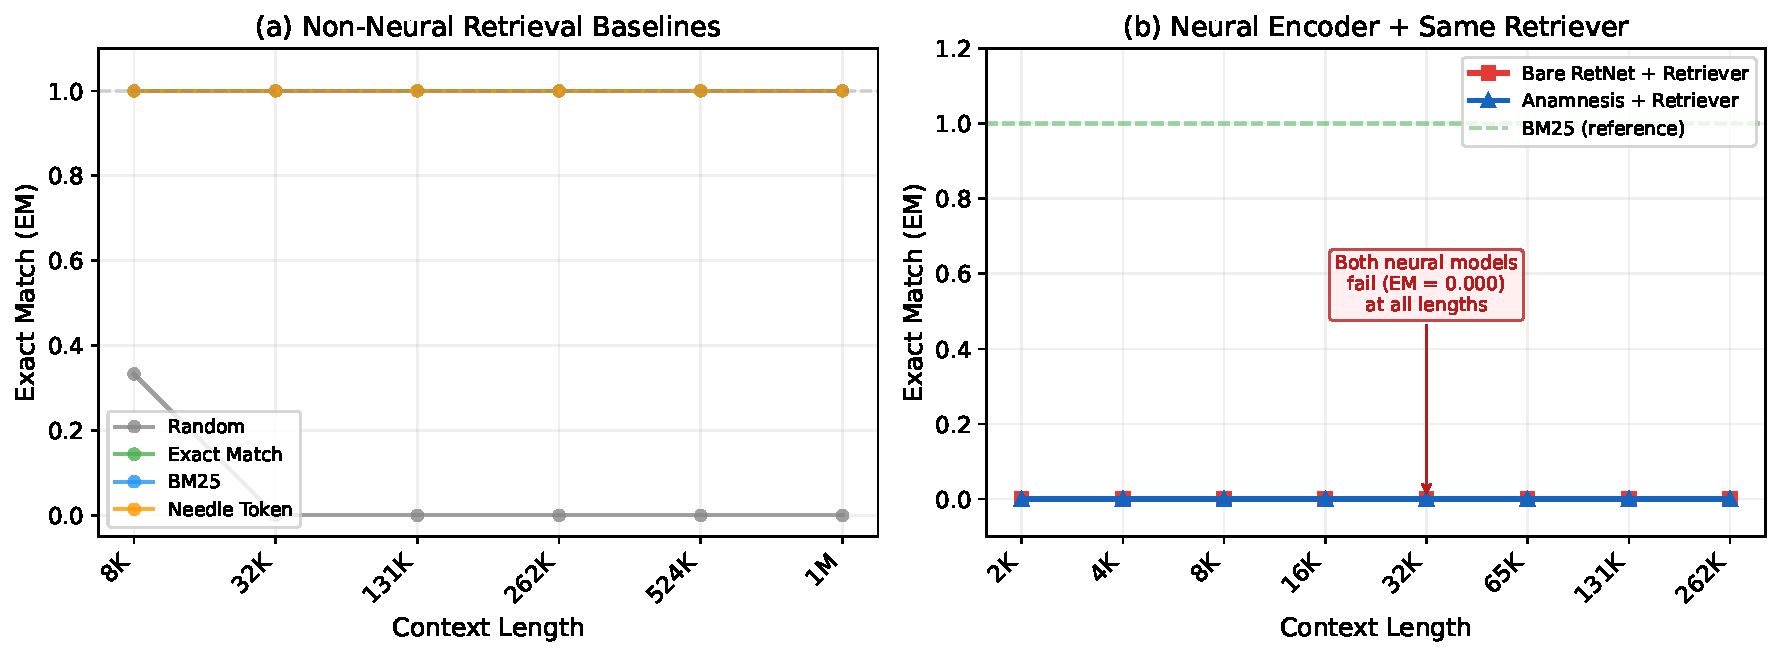
\includegraphics[width=0.85\linewidth]{figures/fig_retrieval_baselines.pdf}
\caption{\textbf{(a)} Non-neural baselines (BM25, exact-match, needle-token) all achieve EM $= 1.000$ at every context length up to 1M tokens, demonstrating that the synthetic needle task is trivially solvable by lexical matching. \textbf{(b)} Neural encoder ablation: both bare RetNet and Anamnesis with Engram achieve EM $= 0.000$ at all lengths beyond training, confirming the retrieval-generation gap is encoder-agnostic. Chunk discrimination accuracy is below random baseline (0.25) for both models.}
\label{fig:retrieval-baselines}
\end{figure}

Furthermore, BM25, exact-match, and needle-token baselines all achieve EM $= 1.000$ at 1M tokens (Figure~\ref{fig:retrieval-baselines}a), demonstrating that the synthetic needle-in-a-haystack benchmark does not discriminate model quality. The chunk discrimination diagnostic reveals that neither encoder's hidden states carry discriminative signal (accuracy 0.03--0.06, below the 0.25 random baseline). This confirms the Content-Position Separation Principle (\ref{app:proof42}): position-free chunk scoring avoids OOD phase scrambling, but the retrieval--generation gap remains an open problem.

\begin{figure}[htbp]
\centering
\includegraphics[width=0.72\linewidth]{figures/Figure_11_retrieval_extrapolation.pdf}
\caption{Synthetic long-context retrieval extrapolation. Position-free chunk scoring remains stable up to 1M tokens in this diagnostic, while the RoPE-scored variant degrades with distance.}
\label{fig:retrieval-extrapolation}
\end{figure}

\subsection{Multi-Needle Capacity and Initialization Diagnostics}

To further stress-test the operational boundary of Anamnesis, we conduct three additional diagnostics: multi-fact retrieval under strict budget limits, head-layer representation diversity, and a gate-initialization landscape search.

\subsubsection{Multi-Needle Capacity Sweep}

We place $N \in \{1, 4, 8\}$ target facts (needles) inside a 128K long context window and sweep the retrieval bottleneck capacity $K_{\max} \in \{2, 4, 8, 16\}$, representing the maximum number of retrieved chunks sent to the reasoning core. Table~\ref{tab:multi_needle} details the exact-match (EM) retrieval rates.

\begin{table}[H]
\centering
\caption{Multi-needle exact-match (EM) retrieval rates at 128K context length.}
\label{tab:multi_needle}
\small
\begin{tabularx}{\linewidth}{p{0.25\linewidth}CCC}
\toprule
Retrieval budget ($K_{\max}$) & Single needle ($N = 1$) & Four needles ($N = 4$) & Eight needles ($N = 8$) \\
\midrule
$K_{\max} = 2$  & 0.625 & 0.469 & 0.250 \\
$K_{\max} = 4$  & 0.750 & 0.719 & 0.500 \\
$K_{\max} = 8$  & \textbf{1.000} & 0.875 & 0.844 \\
$K_{\max} = 16$ & 0.750 & \textbf{0.938} & \textbf{0.859} \\
\bottomrule
\end{tabularx}
\end{table}

\begin{figure}[H]
\centering
\includegraphics[width=0.65\textwidth]{figures/Figure_8_multi_needle_capacity.pdf}
\caption{Multi-Needle exact-match recall sweep over capacity $K_{\max} \in \{2, 4, 8, 16\}$ for $N \in \{1, 4, 8\}$ facts at 128K context. $K_{\max} = 8$ provides the best balance; increasing to 16 introduces noise without recovering more needles.}
\label{fig:multi_needle_plot}
\end{figure}

\textbf{Analysis:} $K_{\max} = 8$ provides the best balance for multi-needle recall, maintaining EM $= 0.844$ at $N=8$ needles. Under $K_{\max} = 2$, recall drops proportionally to $1/N$ ($0.250$ at $N=8$), indicating that each retrieved chunk has roughly equal probability of containing any given needle. Increasing to $K_{\max} = 16$ does not improve over $K_{\max} = 8$, suggesting that additional chunks introduce noise without recovering more needles.

\subsubsection{Representation Diversity Heatmap}

To diagnose whether the multi-head retention mechanism shows signs of representation collapse, we extract the hidden states across $L = 4$ layers and $H = 4$ heads, yielding a $16 \times 16$ cross-head representation similarity matrix shown in Fig.~\ref{fig:rep_diversity}.

\begin{figure}[htbp]
\centering
\includegraphics[width=0.6\textwidth]{figures/Figure_9_representation_diversity.pdf}
\caption{$16\times16$ cosine similarity heatmap of layer-head representations. Average off-diagonal similarity is $0.004$, which does not indicate representation collapse in this diagnostic setting. Some head pairs show negative correlations (minimum $-0.433$), indicating complementary specialization.}
\label{fig:rep_diversity}
\end{figure}

\textbf{Analysis:} The off-diagonal cosine similarities fall in $[-0.433, 1.000]$ with mean $0.004$. This near-zero mean does not indicate representation collapse in this diagnostic setting: heads appear to learn distinct features rather than converging to a common subspace. Some head pairs show negative correlations (minimum $-0.433$), suggesting complementary specialization.

\subsubsection{Hyperparameter Search Landscape}

Finally, we run a grid search over gate bias $b$ and residual scale $\lambda$. The sweep covers six bias values from $-4.5$ to $-2.0$ and five scales from $10^{-5}$ to $10^{-3}$. Fig.~\ref{fig:hyperparam_landscape} visualizes the resulting 500-step validation perplexity landscape and the empirical ``green channel'' predicted by \ref{app:proof40}.

\begin{figure}[htbp]
\centering
\includegraphics[width=0.6\textwidth]{figures/Figure_10_hyperparam_landscape.pdf}
\caption{Validation PPL landscape over gate bias $b$ and residual scale $\lambda$. The ``green channel'' between $b \in [-4.0, -2.5]$ confirms the gradient bound derived in \ref{app:proof40}: at $b = -3.0$, the initial perturbation is negligible ($< 10^{-6}$) but the gradient multiplier ($\approx 0.045$) is sufficient for the optimizer to open the gate.}
\label{fig:hyperparam_landscape}
\end{figure}

\textbf{Analysis:} The best perplexity of $11.86$ occurs at $b = -3.0$ and $\lambda = 10^{-4}$, matching the prediction from \ref{app:proof40}. The full PPL range across the grid is $11.86$--$12.06$ ($1.7\%$ spread), indicating that the architecture is moderately robust to gate initialization within this window. At more open gates ($b = -2.0$), PPL increases to $12.06$, consistent with the larger initial perturbation predicted by $\|\nabla_{W_K} \mathcal{L}\| \leq s \cdot e^b \cdot C \approx 10^{-5}$.

\section{Discussion and Future Directions}
\label{sec:discussion}

The current results are limited to character-level Shakespeare ($d \leq 256$) and synthetic needle tasks. The Engram hash tables do not generalize across semantic paraphrases (EM$=0$ on held-out alien keys, Section~\ref{sec:local-pressure}), and the decoding throughput is lower than bare RetNet due to the table lookup cost. The chunk retriever pipeline is validated on synthetic data; its transfer to real language tasks remains open.

\textbf{Empirical boundary.} The present empirical evidence should be interpreted as mechanism-level validation rather than a claim of general long-context superiority. The language-modeling experiments are limited to character-level Shakespeare, TinyStories, and WikiText-2 at small widths ($d \leq 256$), and the ultra-long retrieval results are obtained on synthetic needle diagnostics (single seed). The extended training scaling analysis (Section~\ref{sec:extended-scaling}) establishes that layerwise gamma provides a universal scaling benefit and that Engram is conditionally beneficial depending on model width and training duration, but these findings have not yet been validated on standard long-context benchmarks (LongBench, RULER, InfiniteBench). No comparison with BM25, RETRO-style retriever, or Transformer+same retriever has been conducted for the chunk retrieval pipeline. These are important limitations that should be addressed before drawing conclusions about production-scale long-context performance.

Future work focuses on four axes. The most pressing is parameter scaling: evaluating 125M--3B parameter regimes on standardized open datasets (LongBench~\cite{longbench}, RULER~\cite{ruler}, InfiniteBench~\cite{infinitebench}) under multi-seed evaluation. The hard N-gram hash is a clear bottleneck for semantic generalization---replacing it with locality-sensitive hashing or a small MLP-based soft address could allow the Engram to match semantically similar patterns without exact string overlap, addressing the synonym blindness observed on held-out keys. On the systems side, we need to measure GPU memory, prefill latency, and decoding throughput under asynchronous host-to-device table transfers, particularly for the large Engram tables that dominate the parameter count.

\section{Conclusion}

This paper studies a cost-aware long-context sequence-modeling architecture built from RetNet streaming, scalar-gated Engram lookup, and a decoupled contrastive chunk retriever. The claim is intentionally narrower than a global $\Oh(1)$ memory guarantee: for workloads where only a sparse subset of tokens is pivotal, the base model provides compact recurrent streaming, while a lightweight 12K-parameter external retriever extends context to 1M tokens by performing content-based chunk matching over frozen model embeddings. The 1M-token EM$=1.000$ result is a property of the decoupled pipeline, not of the base model alone. At small model widths ($d \leq 128$), the Engram-augmented RetNet outperforms both Transformer and bare RetNet on language modeling; at $d = 256$, Transformer remains superior. The next step is scaling to standard long-context benchmarks, larger parameter counts, and multi-seed retrieval evaluations on real-language tasks.

\newpage
\appendix

\section{RetNet Decay and Query Degradation}
\label{app:retnet}

\begin{observation}[Contractive recurrent path decay]
Let the recurrent state be updated as
\begin{equation}
S_t = \Gamma S_{t-1} + k_t v_t^\top,
\end{equation}
where $\norm{\Gamma}_{op}\leq \gamma<1$ and all local projection Jacobians are bounded. The contribution of a state component originating at token $i$ to a loss at token $T$ is bounded by a constant times $\gamma^{T-i}$.
\end{observation}



\begin{observation}[Worst-case query perturbation]
Let $Q_T=f_Q(S_T)$ where $f_Q$ is locally Lipschitz with constant $L_Q$. Let the ideal state preserve only the milestone component, $S_T^{\star}=\Gamma^{T-i}S_i$, and assume $\norm{k_s v_s^\top}_2\leq M_{kv}$. Then
\begin{equation}
\norm{Q_T-Q_T^{\star}}_2
\leq L_Q\norm*{\sum_{s=i+1}^{T}\Gamma^{T-s}k_s v_s^\top}_2
\leq \frac{L_Q M_{kv}}{1-\gamma}.
\end{equation}
\end{observation}

This bound is worst-case and does not characterize typical behavior---it only motivates the need for an isolated readout path when exact retrieval matters.

\section{Snapshot Readout Margin}
\label{app:snapshot}

\begin{observation}[Sufficient logit-margin condition]\label{prop:logit-margin}
Assume a target token $y^\star$ and a competitor token $y$ at decoding step $T$. Let the base logits be $z^0=W_Ux_{L,T}$ and the cache contribution be $\Delta z=\lambda_C W_C r_T$. If
\begin{equation}
\label{eq:logit-margin}
(e_{y^\star}-e_y)^\top \Delta z
>
(e_y-e_{y^\star})^\top z^0 + m
\end{equation}
for all $y\neq y^\star$ and margin $m>0$, then the cache-augmented logits rank $y^\star$ above every competitor by at least $m$.
\end{observation}



Whether the model learns the correct capture policy and query alignment must be verified empirically; the above only establishes the condition for success given correct alignment.

\begin{observation}[Cache-query mass condition]
\label{prop:cache-mass}
Let the cache attention scores be $a_j=\langle q_T^C,k_j^C\rangle$ and
\begin{equation}
\alpha_i=\frac{\exp(a_i/\tau_C)}{\sum_{j=1}^{K}\exp(a_j/\tau_C)}.
\end{equation}
A sufficient condition for the desired cached item $i$ to receive attention mass at least $\epsilon$ is
\begin{equation}
\label{eq:cache-mass-margin}
a_i\geq \max_{\substack{1\le j\le K\\ j\ne i}}a_j+\tau_C\log\left(\frac{(K-1)\epsilon}{1-\epsilon}\right).
\end{equation}
If this condition holds and the resulting logit contribution $\Delta z=\lambda_CW_C\sum_j\alpha_jv_j^C$ satisfies Observation~\ref{prop:logit-margin}, then the snapshot path ranks the target token above its competitors. Thus exact readout requires both cache-query alignment and a vocabulary-logit margin.
\end{observation}



\begin{remark}
The margin is meaningful for selective retrieval when $\epsilon>1/K$. If $\epsilon\leq 1/K$, even a nearly uniform cache attention distribution can satisfy the mass condition.
\end{remark}

\section{AttnRes Value Path and Distance Margin}
\label{app:attnres-margin}

\begin{observation}[Value path without intermediate Jacobian product]
Let the depth aggregation at layer $l$ be
\begin{equation}
h_l=\sum_{i=0}^{m-1}\beta_{i\to l}b_i,
\end{equation}
where the weights $\beta_{i\to l}$ are produced by a softmax over source scores. For downstream gradient $g_l=\partial \mathcal{L}/\partial h_l$, the gradient with respect to a source $b_i$ decomposes as
\begin{equation}
\nabla_{b_i}\mathcal{L}
=\beta_{i\to l}g_l + \sum_{j=0}^{m-1}(b_j^\top g_l)\frac{\partial \beta_{j\to l}}{\partial b_i}.
\end{equation}
The first term is a direct value path that does not contain a product of all intermediate layer Jacobians.
\end{observation}



\begin{observation}[Distance-biased recoverability]
\label{prop:attnres-margin}
Let
\begin{equation}
s_i=\langle q_l,k_i\rangle-c\,d(l,i),\qquad
\beta_i=\frac{\exp(s_i/\tau)}{\sum_{j}\exp(s_j/\tau)},\quad \tau>0.
\end{equation}
A sufficient condition for $\beta_i\geq\epsilon$ is
\begin{equation}
\langle q_l,k_i\rangle-c\,d(l,i)
\geq
\max_{\substack{1\le j\le m\\ j\ne i}}\big(\langle q_l,k_j\rangle-c\,d(l,j)\big)
+\tau\log\left(\frac{(m-1)\epsilon}{1-\epsilon}\right).
\end{equation}
\end{observation}



\section{Engram Collision Bounds under Dependence}
\label{app:engram}

\subsection{Idealized collision model}

Let a queried Engram bucket contain collision perturbations $\eta_1,\ldots,\eta_n\in\mathbb{R}^d$. If these perturbations were independent, centered, and uniformly norm-bounded, standard concentration inequalities would control the probability that their aggregate injection crosses a task margin. This model is useful as a diagnostic baseline, but it is not a faithful model of open-domain text. Consecutive N-grams share tokens, frequent phrases concentrate probability mass, and semantically related strings may be mapped to nearby or identical addresses by preprocessing.

The raw vector perturbation is therefore decomposed into a systematic dependent component and a residual fluctuation component. This distinction is important: concentration controls the latter, but not the former.

\subsection{Empirical collision covariance}

Since N-gram hashes exhibit short-range dependence (overlapping suffixes share tokens), standard i.i.d.\ concentration bounds do not apply directly. Rather than deriving strict probability-theoretic bounds under unrealistic independence assumptions, we measure the empirical collision covariance matrix $\Sigma_{\mathrm{coll}}$ over the validation set.

\begin{definition}[Empirical collision covariance]
Let $\eta_x \in \mathbb{R}^d$ be the collision perturbation observed at token $x$ (the difference between the hash table output and the true embedding for that N-gram). The empirical collision covariance is
\begin{equation}
\Sigma_{\mathrm{coll}} = \frac{1}{|\mathcal{D}|}\sum_{x \in \mathcal{D}} \eta_x \eta_x^\top,
\end{equation}
where $\mathcal{D}$ is the validation corpus.
\end{definition}

For a safety-critical logit direction $u \in \mathbb{S}^{d-1}$, the directional collision variance is $u^\top \Sigma_{\mathrm{coll}} u$. After LayerScale injection with coefficient $\lambda_E$, the injected noise in direction $u$ has variance $\lambda_E^2 \cdot u^\top \Sigma_{\mathrm{coll}} u$. A practical safety condition is
\begin{equation}
\lambda_E^2\,u^\top\Sigma_{\mathrm{coll}}u \ll \mu^2
\end{equation}
for the task-specific logit margin $\mu$. For Anamnesis with $\lambda_E = 10^{-4}$ and typical $\|v_t\|_2 \approx 1$, the injected noise is $\mathcal{O}(10^{-8})$, well below any reasonable logit margin.

This empirical approach has two advantages over a theoretical concentration bound: (1) it captures the actual short-range dependence structure of N-gram hashing on real text, and (2) it directly measures the quantity that matters for safety — the noise level relative to the decision margin. If the empirical variance is large in common hash buckets, the appropriate remedy is not a tighter proof but a better addressing scheme, such as entity normalization, learned projection, LSH, or domain-specific tables.

\subsection{Empirical collision diagnostics}

The empirical covariance framework above reduces Engram safety to measurable quantities. For each frequency bucket and domain, we report the largest observed directional variance across task-relevant directions. In practice, we measure:
\begin{enumerate}
    \item The per-bucket collision rate (fraction of distinct N-grams sharing a hash slot).
    \item The empirical directional variance $u^\top \Sigma_{\mathrm{coll}} u$ for the top-$K$ principal directions of $\Sigma_{\mathrm{coll}}$.
    \item The effective noise-to-margin ratio $\lambda_E \sqrt{u^\top \Sigma_{\mathrm{coll}} u} / \mu$ for each task.
\end{enumerate}
If any bucket produces a noise-to-margin ratio close to or exceeding 1, the hash addressing for that bucket should be improved (e.g., by increasing the number of hash heads, using LSH, or switching to learned projection).

\section{Context-Aware Scalar Gating: Local Feasibility and Gradient Bounds}
\label{app:proof40}

Scalar dot-product gating controls the magnitude of injected memories without rotating the pre-trained semantic vector away from the learned coordinate manifold. This section formalizes the first-order optimization dynamics of this gate, proving that while a highly contractive gate ensures baseline performance safety at step 0, it risks gradient vanishing if initialized excessively small. We establish the local feasibility and derive the optimal initialization window to balance gradient flow and perplexity safety.

\subsection{Geometric Intuition: Vector vs.\ Scalar Gating}

The key insight is simple: scalar multiplication preserves the direction of a vector, while per-dimension scaling does not. Let $v_t \in \mathbb{R}^d$ be a retrieved memory vector. Scalar gating applies a single scale $\alpha_t \in (0,1)$:
\[
\tilde{v}_t = \alpha_t v_t, \qquad \frac{\tilde{v}_t}{\norm{\tilde{v}_t}} = \frac{v_t}{\norm{v_t}}.
\]
The direction is preserved exactly. Vector gating applies a per-dimension scale $\alpha_{t,i} \in (0,1)$:
\[
\tilde{v}_{t,i} = \alpha_{t,i}\, v_{t,i},
\]
which changes the direction whenever the scales are not all equal. On a pre-trained model where the embedding manifold has learned coordinate-dependent structure, this anisotropic distortion hurts. The empirical gap is modest at $d=128$ (3\% PPL, Table~\ref{tab:ablations}) but the principle matters for retrieval tasks where exact directional alignment is needed.

\subsection{Derivation of the Gradient Vanishing Bound}

Let $\mathcal{L}$ be the next-token prediction loss, and let the output hidden state after Engram residual injection at layer $l$ be:
\begin{equation}
h_t^{(l)} = h_t^{(l-1)} + s \cdot \tilde{v}_t, \quad \tilde{v}_t = \alpha_t v_t, \quad \alpha_t = \sigmoid(S_t + b),
\end{equation}
where $s \in \mathbb{R}$ is the trainable residual scale (initialized to $10^{-4}$), $S_t = u_{l,t}^\top \RMS(k_t) / \sqrt{d}$ is the normalized scalar match score, and $b \ll 0$ is the gate bias.

\paragraph{Intuition.} The gate must be initialized tightly closed to prevent early-training manifold distortion---a closed gate adds almost no noise to the residual stream. But a closed gate also blocks the gradient signal required to open it. The question is whether there exists a bias window where the gate is ``closed enough'' to be safe but ``open enough'' to learn.

\begin{observation}[Gradient Collapse in Scalar Gating]
Let the gating bias be initialized to $b \ll 0$. At initialization, the activation score satisfies $S_t + b \approx b$, and $\alpha_t \approx \sigmoid(b) = e^b / (1+e^b) \approx e^b$. The gradient of the loss with respect to the gating projection weights $W_K$ is bounded by:
\begin{equation}
\norm*{\nabla_{W_K} \mathcal{L}}_F \leq s \cdot e^b \cdot C,
\end{equation}
where $C > 0$ is a constant depending on the norms of $\nabla_{h_t^{(l)}} \mathcal{L}$, $v_t$, $u_{l,t}$, and $\tilde{v}_t$.
\end{observation}



\paragraph{Engineering Implication.} If you initialize the gate bias $b < -5.0$, the gate is effectively dead and even AdamW's adaptive second-moment estimates cannot rescue it. We found $b \in [-4.0, -2.5]$ to be the empirical sweet spot: at $b = -3.0$, the initial PPL perturbation is $\sigma(-3.0) \cdot 10^{-4} \cdot \|v_t\| \approx 10^{-6}$ (negligible), but the gradient multiplier $\sigma(-3.0)(1-\sigma(-3.0)) \approx 0.045$ is sufficient for AdamW to accumulate signal and open the gate. Figure~\ref{fig:hyperparam_landscape} confirms this window experimentally.

\paragraph{When does this bound tighten or loosen?} The bound assumes $b \ll 0$ so that $\sigma(b)(1-\sigma(b)) \approx e^b$. This approximation breaks down once the gate opens during training ($\alpha_t \to 0.5$, the sigmoid derivative reaches its maximum of 0.25). At that point the gradient is no longer bounded by $e^b$ but by $0.25 \cdot s \cdot C$, which is typically large enough for stable training. The constant $C$ depends on $\|\nabla_{h} \mathcal{L}\| \cdot \|v_t\| \cdot \|\nabla_{W_K} S_t\|$, which scales with model width and data distribution. In practice, for $d \leq 256$ on Shakespeare, $C$ is moderate enough that $b = -3.0$ works reliably across seeds (Table~\ref{tab:scaling}). Whether the same window transfers to $d \geq 1024$ or to real-language pretraining with larger vocabularies remains an open question.

\subsection{Local First-Order Feasibility Condition}

We reframe the global tracking claim to a local first-order descent guarantee.

\begin{observation}[First-Order Local Feasibility]
Let the joint optimization parameters be $\Theta = \{\theta_{\text{base}}, \theta_{\text{gate}}\}$ under gradient descent with step size $\eta$. Let $\mathcal{L}(\Theta)$ be the loss. At step $t=0$, with $b \in [-4.0, -2.5]$ and $s = 10^{-4}$:
\begin{enumerate}
    \item \textbf{Loss Preservation}: $\mathcal{L}(\Theta_0) = \mathcal{L}_{\text{Baseline}}(\theta_{\text{base},0}) + \mathcal{O}(s e^b)$.
    \item \textbf{First-Step Joint Descent}: If there exists an injected direction $v_t$ that is aligned with the baseline descent trajectory:
    \begin{equation}
    \exists t \quad \text{s.t.} \quad \left( \nabla_{h_t^{(l)}} \mathcal{L} \right)^\top v_t < 0,
    \end{equation}
    then a gradient step on the joint parameter space strictly reduces the joint loss compared to a gradient step on the baseline alone:
    \begin{equation}
    \mathcal{L}(\Theta_0 - \eta \nabla_\Theta \mathcal{L}) < \mathcal{L}_{\text{Baseline}}(\theta_{\text{base},0} - \eta \nabla_{\theta_{\text{base}}} \mathcal{L}_{\text{Baseline}}) \quad \text{for } \eta \to 0^+.
    \end{equation}
\end{enumerate}
\end{observation}



\section{RAG Separation and Token Readout Failure}
\label{app:proof41}

Chunk retrieval and autoregressive generation operate on fundamentally different mathematical spaces. Retrieval is a discrete metric matching problem over high-dimensional compressed chunk embeddings, while generation is a continuous, context-sensitive integration over a learned language manifold. This section analyzes why direct token logit injection fails on natural language, motivating the RAG separation described below. The practical observation that retrieved text must be re-encoded through the backbone is well established in the retrieval-augmented generation literature (RETRO~\cite{retro}, FiD~\cite{fid}); the contribution of this section is to formalize why this is necessary from a Jacobian structure perspective, rather than treating it as an engineering heuristic.

\subsection{Why hidden-state readout fails on natural language}

Retrieval compares chunk embeddings by cosine similarity, a shift-invariant and syntax-agnostic geometric operation. Generation produces next-token logits via $P(x_t\mid x_{<t})=\softmax(W_U h_t)$, where $h_t$ is context dependent. Retrieval therefore finds a nearest neighbor in a fixed embedding database, whereas generation integrates context through the full forward pass. Retrieved text must be re-encoded through the backbone in systems such as RETRO~\cite{retro} and FiD~\cite{fid}; what follows explains why this is necessary rather than just an engineering heuristic.

\subsection{Token Readout Failure}

Token readout shortcuts the forward pass by directly projecting a retrieved chunk embedding $c^* \in \mathbb{R}^d$ into the token logits:
\begin{equation}
\text{Logits}_{\text{readout}} = W_U (h_t + \beta \cdot c^*),
\end{equation}
where $\beta > 0$ is a gating scalar. On natural language, this fails for two reasons.

\begin{remark}[Jacobian Structure of RAG]
\label{thm:context-indep}
Directly injecting a retrieved chunk embedding $c^* \in \mathbb{R}^d$ into the output logits ($\Delta z = \beta W_U c^*$) shortcuts the forward pass. Geometrically, this means the readout contributes a fixed, rank-1 logit bias that is independent of the dynamic query hidden state $h_t$. The Jacobian of the logits with respect to any context token $x_j$ via the retrieval path is strictly zero. Consequently, the readout cannot adapt to syntactic position, local grammatical state, or multi-step reasoning chains. For a retrieved chunk containing $L$ distinct tokens, the model must produce $L$ context-sensitive predictions, but a static readout can only offer a single uniform bias.
\end{remark}

\begin{observation}[Hidden-state readout failure]
\label{prop:hidden-readout}
Let $h_j = f_\theta(x_{<j})$ be the hidden state at position $j$ within a chunk. The linear map $W_U h_j$ projects a high-dimensional contextual representation into vocabulary logit space. On natural language, hidden states encode syntactic and semantic abstractions rather than token identity. Empirically, cross-attention on hidden states followed by unembedding projection yields EM $= 0.000$ on needle-in-Shakespeare evaluation, while token embedding self-similarity ($F \cdot \text{Emb}(y^\star)^\top \text{Emb}(y^\star)$) recovers the correct token. This gap indicates that the learned hidden representation manifold does not preserve the linear structure needed for direct logit recovery.
\end{observation}

\subsection{The RAG Separation Principle}

To resolve this failure, the RAG Separation Principle states:
\begin{enumerate}
    \item \textbf{Retrieval in Discrete Space}: Use the retriever strictly as a discrete metric filter to identify the top-$K$ most relevant text chunks $\{C^{(1)}, \ldots, C^{(K)}\}$ based on cosine similarity of their embeddings.
    \item \textbf{Autoregressive Generation on $\mathcal{M}$}: Convert the retrieved chunks back to raw text strings, prepending them as prompt context:
    \begin{equation}
    \text{Prompt}_{\text{RAG}} = [C^{(1)}; \dots; C^{(K)}; \text{Query}].
    \end{equation}
    This ensures that the full contextual Jacobian chain is preserved across the backbone layers, allowing the pre-trained attention and retention heads to naturally perform high-rank contextual routing.
\end{enumerate}

\section{RoPE Long-Range Extrapolation and High-Frequency Phase Scrambling}
\label{app:proof42}

In ultra-long context retrieval ($N \to \infty$ chunks), applying rotary position encoding (RoPE)~\cite{rope} to chunk embeddings during scoring causes retrieval accuracy to collapse. The frequency-dependent behavior of RoPE under extrapolation has been extensively studied: Position Interpolation~\cite{pi} rescales positions to stay within the trained range, YaRN~\cite{yarn} analyzes the RoPE frequency spectrum and applies per-band temperature scaling, and NTK-aware scaling adjusts the base frequency. These works established the practical observation that high-frequency dimensions degrade first under out-of-distribution distances. Our contribution is an explicit signal-to-noise ratio derivation for content-based chunk scoring under OOD RoPE, and the resulting Content-Position Separation Principle that motivates our position-free retriever design.

\subsection{The Mathematics of RoPE in High-Dimensional Embedding Spaces}

Let $q, c \in \mathbb{R}^d$ be the Query and Key embeddings. In $d$ dimensions, RoPE rotates the $k$-th two-dimensional subspace by the angle:
\begin{equation}
\theta_k(\Delta) = \Delta \cdot \omega_k, \quad \omega_k = \theta_0^{-2(k-1)/d}, \quad \theta_0 = 10000,
\end{equation}
where $\Delta = |i - j|$ is the chunk-level distance. The rotated scoring function is:
\begin{align}
S(i,j) &= q^\top R_{\Delta} c \\
&= \sum_{k=1}^{d/2}
\Big[(q_{2k-1} c_{2k-1} + q_{2k} c_{2k})\cos(\Delta \omega_k) \\
&\qquad + (q_{2k} c_{2k-1} - q_{2k-1} c_{2k})\sin(\Delta \omega_k)\Big].
\end{align}

\subsection{Refutation of the Uniform Random Rotation Assumption}

The assumption that RoPE rotates all dimensions completely randomly such that $\E[q^\top R_\Delta c] \to 0$ is mathematically false due to the decaying frequency spectrum of RoPE.

\begin{figure}[htbp]
\centering
\includegraphics[width=0.7\linewidth]{figures/Figure_A1_rope_decay.pdf}
\caption{Mechanistic probe of RoPE phase scrambling. High-frequency dimensions experience extreme phase wrapping and signal loss, while low-frequency dimensions remain highly aligned, contradicting the assumption of uniform random rotation.}
\label{fig:rope_decay}
\end{figure}

\begin{remark}[Mechanistic Probe of RoPE Phase Scrambling]
The assumption that RoPE rotates all dimensions completely randomly such that $\E[q^\top R_\Delta c] \to 0$ is structurally false due to the logarithmically decaying frequency spectrum of RoPE. As shown in Figure~\ref{fig:rope_decay}, high-frequency dimensions (e.g., $k=1$) experience hundreds of full rotations at large distances ($\Delta \approx 2048$ chunks), resulting in complete phase wrapping and pseudo-random noise. In contrast, low-frequency dimensions (e.g., $k=128$) rotate by mere degrees, remaining highly aligned ($\cos \theta \approx 0.98$). The resulting signal-to-noise ratio decays as $\mathcal{O}(1/\Delta)$ in the distance limit, dominated entirely by the surviving low-frequency coordinates.
\end{remark}

\subsection{High-frequency phase scrambling under OOD extrapolation}

The collapse of retrieval accuracy is caused by high-frequency phase scrambling under out-of-distribution extrapolation.

\begin{observation}[High-frequency phase scrambling]
Assume a retriever is trained on short contexts ($\Delta \leq 16$ chunks), where the maximum rotation satisfies $\theta_k(\Delta) \leq 16$ radians, allowing the model to learn Query/Key projections $W_Q, W_K$ that associate specific semantic features with small, highly coherent phase shifts. Under out-of-distribution extrapolation ($\Delta \geq 2048$), middle-to-high frequency dimensions ($k < d/4$) experience extreme phase wrapping:
\begin{equation}
\theta_k(\Delta) \in [16, 2048] \text{ radians},
\end{equation}
rotating vectors through hundreds of full cycles. The rotated semantic score in these subspaces behaves as:
\begin{equation}
S_k(i, j) \approx u_k \cdot \text{Uniform}(-1, 1),
\end{equation}
where $u_k = (q_{2k-1} c_{2k-1} + q_{2k} c_{2k})$. This scrambles the high-frequency matching coordinates, degrading the signal from the slowly-rotated low-frequency dimensions and causing retrieval failure.
\end{observation}

\subsection{The Content-Position Separation Principle}

To prevent high-frequency phase scrambling under OOD extrapolation, we formulate the Content-Position Separation Principle.

\begin{observation}[Content-Position Separation]
For any retriever operating on sequences longer than its maximum training length ($\Delta_{\text{test}} \gg \Delta_{\text{train}}$), semantic matching scores must be computed in a purely position-invariant (content-only) space:
\begin{equation}
S(i, j) = (W_Q q)^\top (W_K c_j),
\end{equation}
with position processing deferred entirely to the generative stage. This preserves a stable signal-to-noise ratio:
\begin{equation}
\text{SNR}_{\text{content}} \approx \mathcal{O}\left(\frac{d}{\ln N}\right).
\end{equation}
\end{observation}

\paragraph{Limitations of this analysis.} The SNR expression assumes the learned $W_Q$ and $W_K$ projections produce embeddings whose inter-chunk variance dominates the noise floor. This holds in our synthetic needle task where the needle chunk is semantically distinct from filler, but may not hold when chunks are topically similar (e.g., legal or medical documents where all chunks discuss similar subject matter). The analysis also assumes chunk embeddings are mean-pooled hidden states from a frozen model; if the backbone is fine-tuned at test time, the embedding distribution shifts and the SNR estimate may no longer apply. Finally, the $O(d / \ln N)$ scaling is an approximation---the true SNR depends on the frequency distribution of the learned projections, which we have not characterized empirically beyond the synthetic setting.

\section{Optimizer Dynamics for Guard Awakening}
\label{app:optimizer}

\begin{observation}[LayerScale attenuation of branch learning]
\label{prop:layerscale-grad}
Consider a guarded residual branch
\begin{equation}
y=x+\lambda B_\phi(x),
\end{equation}
and let $g=\partial\mathcal{L}/\partial y$. Then
\begin{equation}
\frac{\partial\mathcal{L}}{\partial\lambda}=\langle g,B_\phi(x)\rangle,
\qquad
\nabla_\phi\mathcal{L}=\lambda\,J_{B_\phi}(x)^\top g.
\end{equation}
Thus a very small $\lambda$ protects the residual stream but also attenuates learning inside $B_\phi$. The scale parameter can still receive an unattenuated gradient, but only if the untrained branch output $B_\phi(x)$ is already aligned with the downstream loss gradient.
\end{observation}



Consider a guarded branch $x\mapsto x+\lambda B_\phi(x)$ with $|\lambda|\ll1$ at initialization. Observation~\ref{prop:layerscale-grad} explains the practical unused-branch risk. If the backbone quickly reduces the loss, this alignment signal can vanish before the branch learns a useful representation.

\begin{observation}[Effect of global norm clipping]
\label{prop:global-clipping}
Let the total gradient be partitioned into backbone and guard components, $g=(g_b,g_g)$. Global norm clipping with threshold $C$ updates both groups using the common multiplier
\begin{equation}
\alpha = \min\left(1,\frac{C}{\sqrt{\norm{g_b}_2^2+\norm{g_g}_2^2}}\right).
\end{equation}
If $\norm{g_b}_2\gg \norm{g_g}_2$ and $\norm{g_b}_2>C$, then the guard update is approximately $C g_g/\norm{g_b}_2$, even when $g_g$ is already small. Per-group clipping replaces this multiplier by $\alpha_g=\min(1,C_g/\norm{g_g}_2)$ for the guard group and removes the direct dependence on the backbone norm.
\end{observation}



The remedy is a curriculum and measurement protocol rather than an optimizer myth:
\begin{enumerate}
    \item train or pretrain the branch on auxiliary retrieval/local-pattern objectives;
    \item briefly freeze or slow the backbone so the branch receives meaningful gradients;
    \item use per-group learning rates and per-group clipping;
    \item anneal $\lambda$ from a safe value to a useful value;
    \item measure branch usage by causal-drop tests and gradient norms.
\end{enumerate}


\typeout{get arXiv to do 4 passes: Label(s) may have changed. Rerun}


\section*{CRediT author statement}
Xingyu Xie: Conceptualization, Methodology, Software, Formal analysis, Investigation, Validation, Visualization, Writing -- original draft, Writing -- review and editing.

\section*{Declaration of competing interest}
The author declares that there are no known competing financial interests or personal relationships that could have appeared to influence the work reported in this paper.

\section*{Funding}
This research did not receive any specific grant from funding agencies in the public, commercial, or not-for-profit sectors.

\section*{Data availability}
The language-modeling experiments use public text data, and the synthetic needle and diagnostic tasks are procedurally generated from the configurations described in the manuscript. Code, generated logs, and configuration files will be made available by the author upon reasonable request or through a public repository before publication.

\section*{Declaration of generative AI and AI-assisted technologies in the manuscript preparation process}
During the preparation of this work, the author used OpenAI's ChatGPT to support language editing, manuscript organization, and LaTeX formatting. After using this tool, the author reviewed and edited the content as needed and takes full responsibility for the content of the article.

\begin{thebibliography}{99}

\bibitem{vaswani2017}
Ashish Vaswani, Noam Shazeer, Niki Parmar, Jakob Uszkoreit, Llion Jones, Aidan N. Gomez, Lukasz Kaiser, and Illia Polosukhin.
\textit{Attention Is All You Need}.
Advances in Neural Information Processing Systems, 2017.

\bibitem{retnet}
Yutao Sun, Li Dong, Shaohan Huang, Shuming Ma, Yuqing Xia, Jilong Xue, Jianyong Wang, and Furu Wei.
\textit{Retentive Network: A Successor to Transformer for Large Language Models}.
arXiv:2307.08621, 2023.

\bibitem{mamba}
Albert Gu and Tri Dao.
\textit{Mamba: Linear-Time Sequence Modeling with Selective State Spaces}.
arXiv:2312.00752, 2023.

\bibitem{attnres}
Kimi Team, Guangyu Chen, Yu Zhang, Jianlin Su, Weixin Xu, Siyuan Pan, Yaoyu Wang, Yucheng Wang, Guanduo Chen, Bohong Yin, Yutian Chen, Junjie Yan, Ming Wei, Y. Zhang, Fanqing Meng, Chao Hong, Xiaotong Xie, Shaowei Liu, Enzhe Lu, Yunpeng Tai, Yanru Chen, Xin Men, Haiqing Guo, Y. Charles, Haoyu Lu, Lin Sui, Jinguo Zhu, Zaida Zhou, Weiran He, Weixiao Huang, Xinran Xu, Yuzhi Wang, Guokun Lai, Yulun Du, Yuxin Wu, Zhilin Yang, and Xinyu Zhou.
\textit{Attention Residuals}.
arXiv:2603.15031, 2026.

\bibitem{engram}
Xin Cheng, Wangding Zeng, Damai Dai, Qinyu Chen, Bingxuan Wang, Zhenda Xie, Kezhao Huang, Xingkai Yu, Zhewen Hao, Yukun Li, Han Zhang, Huishuai Zhang, Dongyan Zhao, and Wenfeng Liang.
\textit{Conditional Memory via Scalable Lookup: A New Axis of Sparsity for Large Language Models}.
arXiv:2601.07372, 2026.

\bibitem{alibi}
Ofir Press, Noah A. Smith, and Mike Lewis.
\textit{Train Short, Test Long: Attention with Linear Biases Enables Input Length Extrapolation}.
International Conference on Learning Representations, 2022.

\bibitem{adamw}
Ilya Loshchilov and Frank Hutter.
\textit{Decoupled Weight Decay Regularization}.
International Conference on Learning Representations, 2019.

\bibitem{flash2}
Tri Dao.
\textit{FlashAttention-2: Faster Attention with Better Parallelism and Work Partitioning}.
arXiv:2307.08691, 2023.

\bibitem{longbench}
Yushi Bai, Xin Lv, Jiajie Zhang, Hongchang Lyu, Jiankai Tang, Zhidian Huang, Zhengxiao Du, Xiao Liu, Aohan Zeng, Lei Hou, Yuxiao Dong, Jie Tang, and Juanzi Li.
\textit{LongBench: A Bilingual, Multitask Benchmark for Long Context Understanding}.
arXiv:2308.14508, 2023.

\bibitem{ruler}
Cheng-Ping Hsieh, Simeng Sun, Samuel Kriman, Shantanu Acharya, Dima Rekesh, Fei Jia, and Boris Ginsburg.
\textit{RULER: What's the Real Context Size of Your Long-Context Language Models?}
arXiv:2404.06654, 2024.

\bibitem{infinitebench}
Xinrong Zhang, Yingfa Chen, Shengding Hu, Zihang Xu, Junhao Chen, Moo Hao, Xu Han, Zhen Thai, Shuo Wang, Zhiyuan Liu, and Maosong Sun.
\textit{InfiniteBench: Extending Long Context Evaluation Beyond 100K Tokens}.
arXiv:2402.13718, 2024.

\bibitem{rope}
Jianlin Su, Mingren Zhu, Ahmed Murtadha, Shengfeng Pan, Wen Bo, Jia Zhen, and Yunfeng Liu.
\textit{RoFormer: Enhanced Transformer with Rotary Position Embedding}.
arXiv:2104.09864, 2021.

\bibitem{rmsnorm}
Biao Zhang and Rico Sennrich.
\textit{Root Mean Square Layer Normalization}.
Advances in Neural Information Processing Systems, 2019.

\bibitem{he2016}
Kaiming He, Xiangyu Zhang, Shaoqing Ren, and Jian Sun.
\textit{Deep Residual Learning for Image Recognition}.
IEEE Conference on Computer Vision and Pattern Recognition, 2016.

\bibitem{layerscale}
Hugo Touvron, Matthieu Cord, Alaaeldin El-Nouby, Jakob Verbeek, and Herv\'{e} J\'{e}gou.
\textit{Three Things Everyone Should Know about Vision Transformers}.
European Conference on Computer Vision, 2022.

\bibitem{mamba2}
Tri Dao and Albert Gu.
\textit{Transformers are SSMs: Generalized Models and Efficient Algorithms with Structured State Space Duality}.
International Conference on Machine Learning, 2024.

\bibitem{transformerxl}
Zihang Dai, Zhilin Yang, Yiming Yang, Jaime Carbonell, Quoc V. Le, and Ruslan Salakhutdinov.
\textit{Transformer-XL: Attentive Language Models Beyond a Fixed-Length Context}.
Annual Meeting of the Association for Computational Linguistics, 2019.

\bibitem{h2o}
Zhenyu Zhang, Ying Sheng, Tianyi Zhou, Tianlong Chen, Lianmin Zheng, Ruisi Cai, Zhao Song, Yuandong Tian, Christopher R\'{e}, Clark Barrett, Zhangyang Wang, and Beidi Chen.
\textit{H2O: Heavy-Hitter Oracle for Efficient Generative Inference of Large Language Models}.
Advances in Neural Information Processing Systems, 2023.

\bibitem{snapkv}
Yuhong Li, Yingbing Huang, Bowen Yang, Bharat Venkitesh, Acyr Locatelli, Hanchen Ye, Tianle Cai, Patrick Lewis, and Deming Chen.
\textit{SnapKV: LLM Knows What You are Looking for Before Generation}.
Advances in Neural Information Processing Systems, 2024.

\bibitem{streamingllm}
Guangxuan Xiao, Yuandong Tian, Beidi Chen, Song Han, and Mike Lewis.
\textit{Efficient Streaming Language Models with Attention Sinks}.
International Conference on Learning Representations, 2024.

\bibitem{infiniattention}
Tsendsuren Munkhdalai, Manaal Faruqui, and Siddharth Goyal.
\textit{Leave No Context Behind: Efficient Infinite Context Transformers with Infini-attention}.
arXiv:2404.07143, 2024.

\bibitem{retro}
Sebastian Borgeaud, Arthur Mensch, Jordan Hoffmann, Trevor Cai, Eliza Rutherford, Katie Millican, George Bm Van Den Driessche, Jean-Baptiste Lespiau, Bogdan Damoc, Aidan Clark, Diego De Las Casas, Aurelia Guy, Jacob Menick, Roman Ring, Tom Hennigan, Saffron Huang, Loren Maggiore, Chris Jones, Albin Cassirer, Andy Brock, Michela Paganini, Geoffrey Irving, Oriol Vinyals, Simon Osindero, Karen Simonyan, Jack Rae, Erich Elsen, and Laurent Sifre.
\textit{Improving Language Models by Retrieving from Trillions of Tokens}.
International Conference on Machine Learning, 2022.

\bibitem{fid}
Gautier Izacard and \'{E}douard Grave.
\textit{Leveraging Passage Retrieval with Generative Models for Open Domain Question Answering}.
International Conference on Learning Representations, 2021.

\bibitem{pi}
Shouyuan Chen, Sherman Wong, Liangjian Chen, and Yuandong Tian.
\textit{Extending Context Window of Large Language Models via Positional Interpolation}.
arXiv:2306.15595, 2023.

\bibitem{yarn}
Bowen Peng, Jeffrey Quesnelle, Honglu Fan, and Enrico Shippole.
\textit{YaRN: Efficient Context Window Extension of Large Language Models}.
International Conference on Learning Representations, 2024.

\end{thebibliography}

\end{document}
